\appendix

\section{Mutual $k$-Nearest Neighbor Alignment Metric}\label{sec:align-metric}
For two models with representations $f$, $g$ the mutual $k$-nearest neighbor metric measures the average overlap of their respective nearest neighbor sets. In this section, we refer to this metric as $m_{\texttt{NN}}$, which we will formally define below.

For cross-modal domains, define $(x_i, y_i) \in \mathcal{X}$ as a sample from the data distribution $\mathcal{X}$ (\eg image-caption dataset). For the single domain alignment measurements, the samples are equivalent $x_i = y_i$ (\eg, images for vision, and text for language). 
Let $\{x_i, y_i\}_{i=1}^{b}$ be the corresponding mini-batch sampled from this data distribution. Then given two model representations $f$ and $g$ the corresponding features are:
$\phi_i =f(x_i)$ and $\psi_i =g(y_i)$, where the collection of these features are denoted as $\Phi = \{ \phi_1, \dots, \phi_b \}$ and $\Psi = \{ \psi_1, \dots, \psi_b \}$. 
Then for each feature pair $(\phi_i, \psi_i)$, we compute the respective nearest neighbor sets $\mathcal{S}(\phi_i)$ and $\mathcal{S}(\psi_i)$. 
\begin{align}
d_{\mathsf{knn}}(\phi_i, \Phi \setminus \phi_i) =  \mathcal{S}(\phi_i) \\
d_{\mathsf{knn}}(\psi_i, \Psi \setminus \psi_i) =  \mathcal{S}(\psi_i)
\end{align}
where $d_{\texttt{knn}}$ returns the set of indices of its $k$-nearest neighbors. Then we measure its average intersection via
\begin{align}
m_{\texttt{NN}}(\phi_i, \psi_i) = \frac{1}{k} \lvert \mathcal{S}(\phi_i) \cap \mathcal{S}(\psi_i) \rvert
\end{align}
where $\lvert {}\cdot{} \rvert$ is the size of the intersection.

\paragraph{The choice to use mutual nearest-neighbors}

Our initial efforts to measure alignment with CKA revealed a very weak trend of alignment between models, even when comparing models within their own modality. This has also been observed by~\cite{bansal2021revisiting}, which had relied on alternative metrics such as model-stitching as it ``reveals aspects of representations that measures such as centered kernel alignment (CKA) cannot''~\cite{bansal2021revisiting}.

We chose to use nearest-neighbor as a metric, as methods like CKA has a very strict definition of alignment, which may not fit our current needs. 
For instance, understanding the precise similarity between unrelated items, such as an orange and Bill Gates, may not be critical.%, or the exact distances among a dog, a cat, and a giant squid, may not be critical. %It's more important to recognize that a dog and cat are more likely to co-occur together than either is to co-occur with a giant squid. 

% For similar reasons, existing works relied on alternative metrics such as model-stitching as it ``reveals aspects of representations that measures such as centered kernel alignment (CKA) cannot''~\cite{bansal2021revisiting}.

\paragraph{Relationship between CKA and Mutual Nearest-Neighbors}

Let $\phi_i \in \mathbb{R}^{n}$ and $\psi_i \in \mathbb{R}^{m}$ be vectorized features of two models (\eg language and vision models). Let $\bK_{ij} = \kappa(\phi_i, \phi_j)$ and $\bL_{ij} = \kappa(\psi_i, \psi_j)$ be the kernel matrices computed from a dataset using some kernel-function $\kappa$. Using an inner-product kernel, the $ij$-th entry of the centered counterpart of these Kernel matrices is:
\begin{align}
\bar{\bK}_{ij} = \langle \phi_i, \phi_j \rangle - \mathbb{E}_l[\langle \phi_i, \phi_l \rangle] \qquad\qquad \bar{\bL}_{ij} = \langle \psi_i, \psi_j \rangle - \mathbb{E}_l[\langle \psi_i, \psi_l \rangle]
\end{align}
Then, the cross-covariance of $\bK$ and $\bL$ is given by:
\begin{align}
\mathsf{HSIC}(\bK, \bL) = \frac{1}{(n-1)^2} \tr (\bar{\bK} \bar{\bL})
\end{align}
which serves as an empirical estimator of the Hilbert-Schmidt Independence Criterion~\cite{gretton2005measuring}. The Centered Kernel Alignment~(CKA)~\cite{kornblith2019similarity} is then its normalized counterpart:
\begin{align}
\mathsf{CKA}(\bK, \bL) = \frac{\mathsf{HSIC}(\bK, \bL)}{\sqrt{\mathsf{HSIC}(\bK, \bK) \mathsf{HSIC}(\bL, \bL)}}
\end{align}
CKA measures the congruence between two random variables, with a maximum alignment of $1$ and a minimum of $0$. It is invariant to isotropic scaling and offers a strict notion of alignment, measuring alignment across all samples. Hence, the CKA score reflects the global similarities of the models. This can be illustrated by expanding the trace term in HSIC:
\begin{align}
\tr(\bar{\bK} \bar{\bL}) = \sum_i \sum_j \left(\langle \phi_i, \phi_j \rangle - \mathbb{E}_l[\langle \phi_i, \phi_l \rangle]\right) \left(\langle \psi_i, \psi_j \rangle - \mathbb{E}_l[\langle \psi_i, \psi_l\rangle]\right)
\end{align}
One can modify the definition of alignment to restrict the cross-covariance measurement to samples considered to be nearest neighbors of the current sample $i$. This emphasizes similarity over dissimilarity, biasing the measure toward local alignment:
% \begin{align}
% \label{eqn:cknna}
% \mathsf{Align_{knn}}(\bK, \bL) = \sum_i \hspace{-0.1in} \sum_{ \substack{ j \in \\ \mathsf{knn}(\phi_i) \\ \cup \mathsf{knn}(\psi_i) }} \hspace{-0.1in} \alpha(i, j) \cdot \left(\langle \phi_i, \phi_j \rangle - \mathbb{E}_l[\langle \phi_i, \phi_l \rangle]\right) \left(\langle \psi_i, \psi_j \rangle - \mathbb{E}_l[\langle \psi_i, \psi_l\rangle]\right)
% \end{align}
\begin{align}
% \label{eqn:cknna}
\mathsf{Align_{knn}}(\bK, \bL) &= \sum_i \sum_j \alpha(i, j) \cdot \left(\langle \phi_i, \phi_j \rangle - \mathbb{E}_l[\langle \phi_i, \phi_l \rangle]\right) \left(\langle \psi_i, \psi_j \rangle - \mathbb{E}_l[\langle \psi_i, \psi_l\rangle]\right) \\
&\text{where} \qquad \alpha(i, j) = \mathbb{1}[\phi_j \in \mathsf{knn}(\phi_i) \land \psi_j \in \mathsf{knn}(\psi_i) \land i \neq j]
\end{align}

\begin{figure*}[t!]
    \centering
    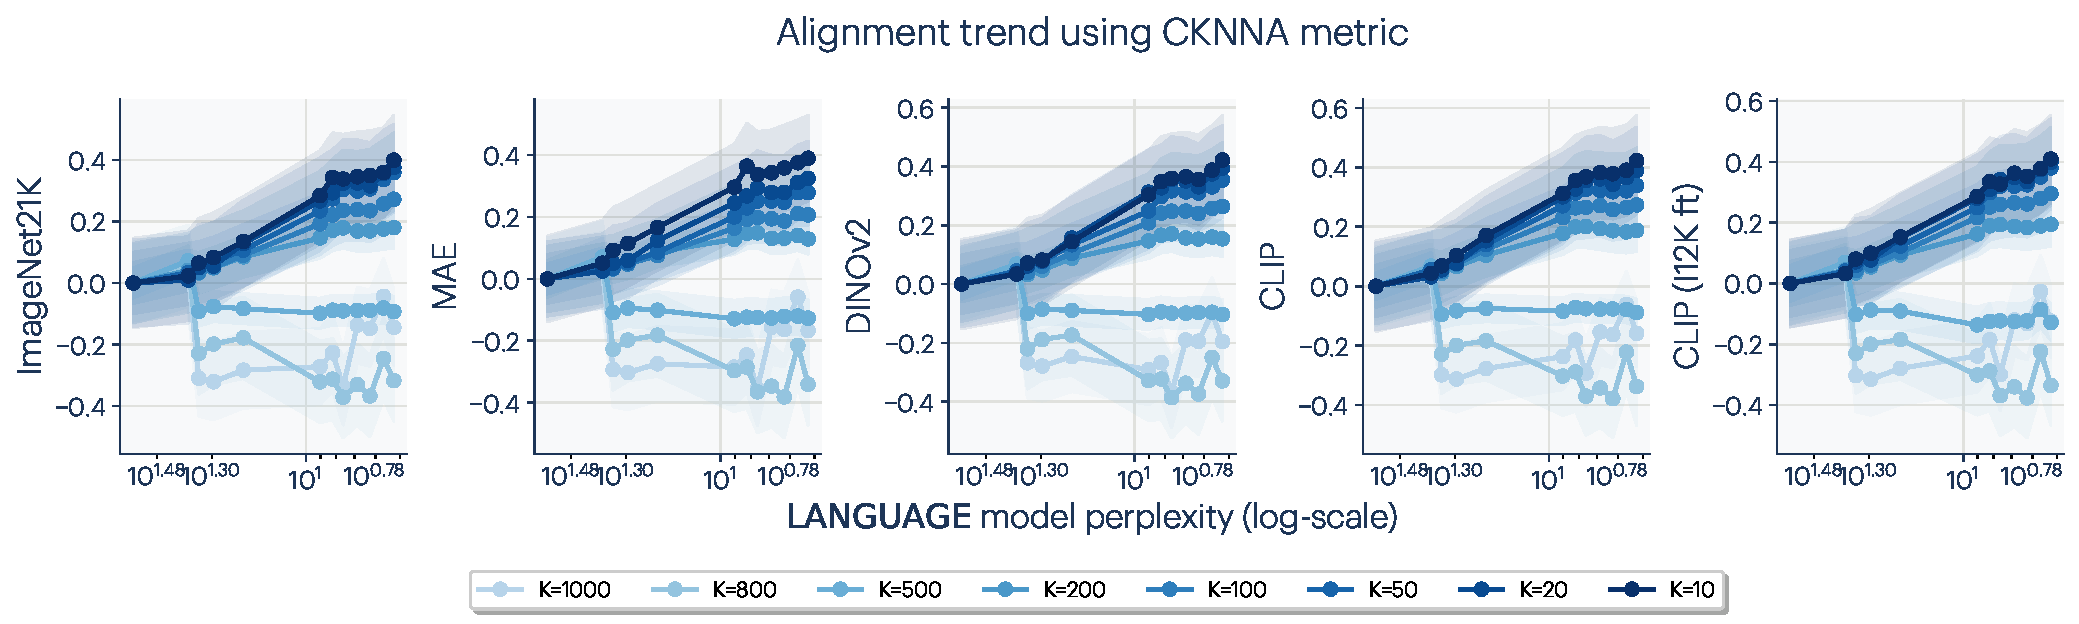
\includegraphics[width=0.98\linewidth]{figures/cknna.pdf}\\
    \caption{\small \textbf{Cross-modal alignment increases locally:} 
    Alignment trend when varying the top-$k$ nearest neighbors in the CKNNA metrics~(\eqn{eqn:cknna}). We center alignment score to the smallest language model and divide the total trend by the standard deviation. When $k=1024$, we recover the original CKA metric, and when $k < | \mathcal{X} |$ it closely resembles the mutual nearest-neighbor metric $m_{\texttt{NN}}$. Each line represents the average of all LLM models for a specific $k$. As we decrease $k$, the alignment becomes more pronounced.}
    \label{fig:cknna}
    \vspace{-3pt}
\end{figure*}

Where $\alpha(i, j)$ is a scalar weighting that assigns $1$ if $j$ is a mutual nearest neighbors to both $\phi_i$ and $\psi_i$, and $0$ otherwise. We refer to this metric as the Centered Kernel Nearest-Neighbor Alignment (CKNNA) metric. As the number of nearest neighbors $k \rightarrow \dim(\bK)$, we recover the original CKA metric. 

\begin{align}
\label{eqn:cknna}
\mathsf{CKNNA}(\bK, \bL) = \frac{\mathsf{Align_{knn}}(\bK, \bL)}{\sqrt{\mathsf{Align_{knn}}(\bK, \bK), \mathsf{Align_{knn}}(\bL, \bL)}}
\end{align}

% The $\mathsf{knn}$ kernels can be efficiently computed by the function $m_{\mathsf{topk}}$, which generates a binary mask that assigns $1$ to the top $k$ elements for each row.
% \begin{align}
% \bK_{\mathsf{knn}} &= \frac{1}{2}\left( m_{\mathsf{topk}}(\bK) + m_{\mathsf{topk}}(\bK)^\T \right) \odot \bK = \bM_{\bK} \odot \bK \\
% \bL_{\mathsf{knn}} &= \frac{1}{2}\left( m_{\mathsf{topk}}(\bL) + m_{\mathsf{topk}}(\bL)^\T \right) \odot \bL = \bM_{\bL} \odot \bL
% \end{align}

We can further relax the metric to treat the cross-covariance term identically across all nearest-neighbor samples. This is equivalent to the assumption that all nearby samples have the same distance. This simplification leads us back to the mutual nearest neighbor metric:
\begin{align}
\sum_i \sum_{j} \alpha(i, j) \cdot 1 = n \cdot k \cdot m_{\texttt{NN}}(\phi_i, \psi_i)
\end{align}


By equating these metrics, we analyze the changes in alignment between language and vision models as we vary the number of neighbors $k$ in \eqn{eqn:cknna}. In \fig{fig:cknna}, we compute the average alignment score across all LLM models. For each $k$, we center the scores to the smallest vision model and divide by the standard deviation of the scores. We find that high values of $k$ show less conclusive alignment across tasks while decreasing $k$ shows a coherent trend across both models and tasks.

\newpage
\section{Consistency across various metrics}
\label{app:other-metrics}

We describe the metrics in~\tbl{tbl:metrics} and their corresponding properties. The \textit{symmetric} property implies that the metric is symmetric with respect to the data points $d(x, y) = d(y, x)$. The \textit{global} property means all samples are used to compute the distance with respect to every sample. The \textit{ordinal} property is when the ordering of the distance is taken into consideration. For example, mutual nearest neighbor is not ordinal since the nearest neighbors $\{a, b, c\}$ and $\{c, a, b\}$ are treated equally. The \textit{batchable} property is a computational property that makes it feasible to compute in a reasonable time frame.

\paragraph{Vision-vision comparison} 
In \Cref{fig:app-same-modal-rankr}, we evaluate Spearman's rank correlation among different metrics and hyperparameters over $78$ vision models (details in \Cref{sec:vision-vision-details}). We find most metrics highly correlated with each other.

\paragraph{Cross-modal comparison} We measure vision-language alignment using a range of alternative metrics.  We visualize the corresponding alignment results in~\fig{fig:metrics1of2} and~\fig{fig:metrics2of2}. Our findings indicate that alignment sensitivity not only depends on the metric used to compute it but also varies according to the specific tasks on which the vision models are trained.

\vspace{0.3in}
\begin{figure}[hbtp]
\centering
\newcommand{\centercell}[1]{\multicolumn{1}{C}{#1}}
\definecolor{lightgray}{gray}{0.9}  
\begin{tabular}{rccccp{8.2cm}} 
    \toprule
    \multirow{2}{*}{\textbf{Metric}} & \multicolumn{4}{c}{\textbf{Property}} & \thead{\multirow{2}{*}{\textbf{Description}}} \\
    \cmidrule(lr){2-6}
    & \small symmetric & \small global & \small ordinal & \small batchable & \\
    \midrule
    \rowcolor{lightgray}
    \multirow{3}{*}[-0.5em]{CKA} & 
    \multirow{3}{*}[-0.5em]{\cmark} & 
    \multirow{3}{*}[-0.5em]{\cmark} & 
    \multirow{3}{*}[-0.5em]{\cmark} & 
    \multirow{3}{*}[-0.5em]{\cmark} & 
    {\vspace{-0.5em}Centered Kernel Alignment~(CKA; \citet{kornblith2019similarity}) measures the similarity of neural networks by comparing the alignment of their kernel induced by their feature spaces.} \\[3.1em]
    \multirow{2}{*}[-0.5em]{Unbiased CKA} & 
    \multirow{2}{*}[-0.5em]{\cmark} & 
    \multirow{2}{*}[-0.5em]{\cmark} & 
    \multirow{2}{*}[-0.5em]{\cmark} & 
    \multirow{2}{*}[-0.5em]{\cmark} & 
    {\vspace{-0.5em}Unbiased estimator of CKA that corrects for sample bias in HSIC~\cite{song2012feature}.} \\[1.8em]
    \rowcolor{lightgray}
    \multirow{4}{*}[-0.5em]{SVCCA} & 
    \multirow{4}{*}[-0.5em]{\cmark} & 
    \multirow{4}{*}[-0.5em]{\cmark} & 
    \multirow{4}{*}[-0.5em]{\cmark} & 
    \multirow{4}{*}[-0.5em]{\cmark} & 
    {\vspace{-0.5em}Singular Value Canonical Correlation Analysis~(SVCCA; \citet{raghu2017svcca}) compares neural networks by decomposing their activities into singular vectors and measuring correlation.} \\[4.2em]
    % \rowcolor{lightgray}
    \multirow{2}{*}[-0.5em]{Mutual $k$-NN} & 
    \multirow{2}{*}[-0.5em]{\cmark} & 
    \multirow{2}{*}[-0.5em]{ } & 
    \multirow{2}{*}[-0.5em]{ } & 
    \multirow{2}{*}[-0.5em]{\cmark} &
    {\vspace{-0.5em}Measures the intersection over union (IoU) of nearest neighbors between two models.} \\[1.8em]
    \rowcolor{lightgray}
    \multirow{2}{*}[-0.5em]{CKNNA} &
    \multirow{2}{*}[-0.5em]{\cmark} &
    \multirow{2}{*}[-0.5em]{\cmark$\ast$} &
    \multirow{2}{*}[-0.5em]{\cmark} &
    \multirow{2}{*}[-0.5em]{\cmark} & 
    {\vspace{-0.5em}Modified CKA measure that computes the kernel alignment only for its nearest neighbors. See~\app{sec:align-metric}.} \\[1.8em]
    % \rowcolor{lightgray}
    \multirow{3}{*}[-0.5em]{Cycle $k$-NN} &
    \multirow{3}{*}[-0.5em]{ } &
    \multirow{3}{*}[-0.5em]{ } &
    \multirow{3}{*}[-0.5em]{ } &
    \multirow{3}{*}[-0.5em]{\cmark} & 
    {\vspace{-0.5em}Measures whether the nearest neighbor in one domain also considers the original sample as its nearest neighbor in the other domain.}  \\[3.1em]
    \rowcolor{lightgray}
    \multirow{3}{*}[-0.5em]{Edit $k$-NN} &
    \multirow{3}{*}[-0.5em]{\cmark} &
    \multirow{3}{*}[-0.5em]{\cmark$\ast$} &
    \multirow{3}{*}[-0.5em]{\cmark} &
    \multirow{3}{*}[-0.5em]{ } & 
    {\vspace{-0.5em}Computes the edit distance required to match the nearest neighbors between two datasets. The score is normalized by the maximum edit distance.} \\[3.1em]
    % \rowcolor{lightgray}
    \multirow{2}{*}[-0.5em]{LCS $k$-NN} &
    \multirow{2}{*}[-0.5em]{\cmark} &
    \multirow{2}{*}[-0.5em]{\cmark$\ast$} &
    \multirow{2}{*}[-0.5em]{\cmark} &
    \multirow{2}{*}[-0.5em]{ } & 
    {\vspace{-0.5em}Calculates the longest common subsequence of nearest neighbors and is normalized by the sequence length.} \\[1.7em]
    \bottomrule
\end{tabular}
\caption{Comparative analysis of neural network similarity metrics. \cmark$\ast$ indicates the metric is global and still meaningful when the nearest neighbor $k$ is set to maximum batch-size $k=|\mathcal{X}|$.}
\label{tbl:metrics}
\end{figure}

\begin{figure*}[hbtp]
    \centering
    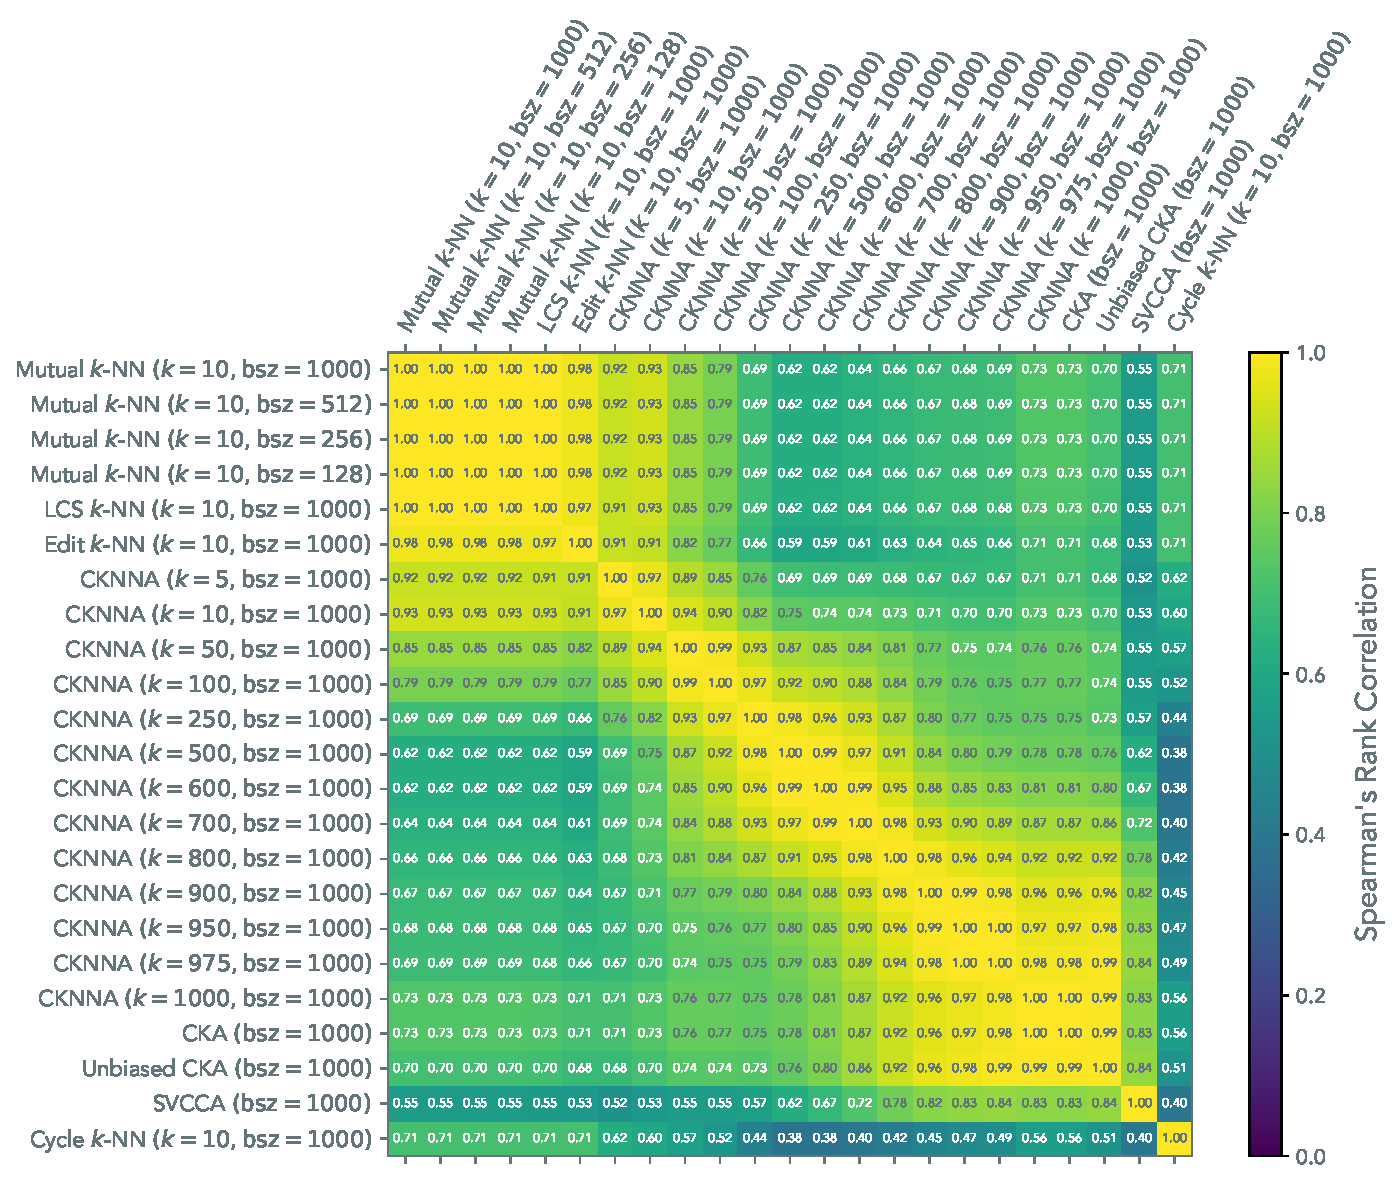
\includegraphics[width=1\linewidth]{figures/vision_metrics_rankr.pdf}
    \caption{\textbf{Vision-vision alignment measured with various metrics.} Spearman's rank correlation among different metrics and batch sizes ($\mathsf{bsz}$) when used to measure alignment among $78$ vision models (see \Cref{sec:vision-vision-details} for details of these models). All $p$-values are below $2.24\times 10^{-105}$. Our vision-vision analysis in \Cref{fig:vm_align} is based on the first metric (Mutual $k$-NN with $k=10$ and $\mathsf{bsz}=1000$).}
    \label{fig:app-same-modal-rankr}
\end{figure*}


\begin{figure*}[hbtp]
    \centering
    \subfigure[CKA]{
        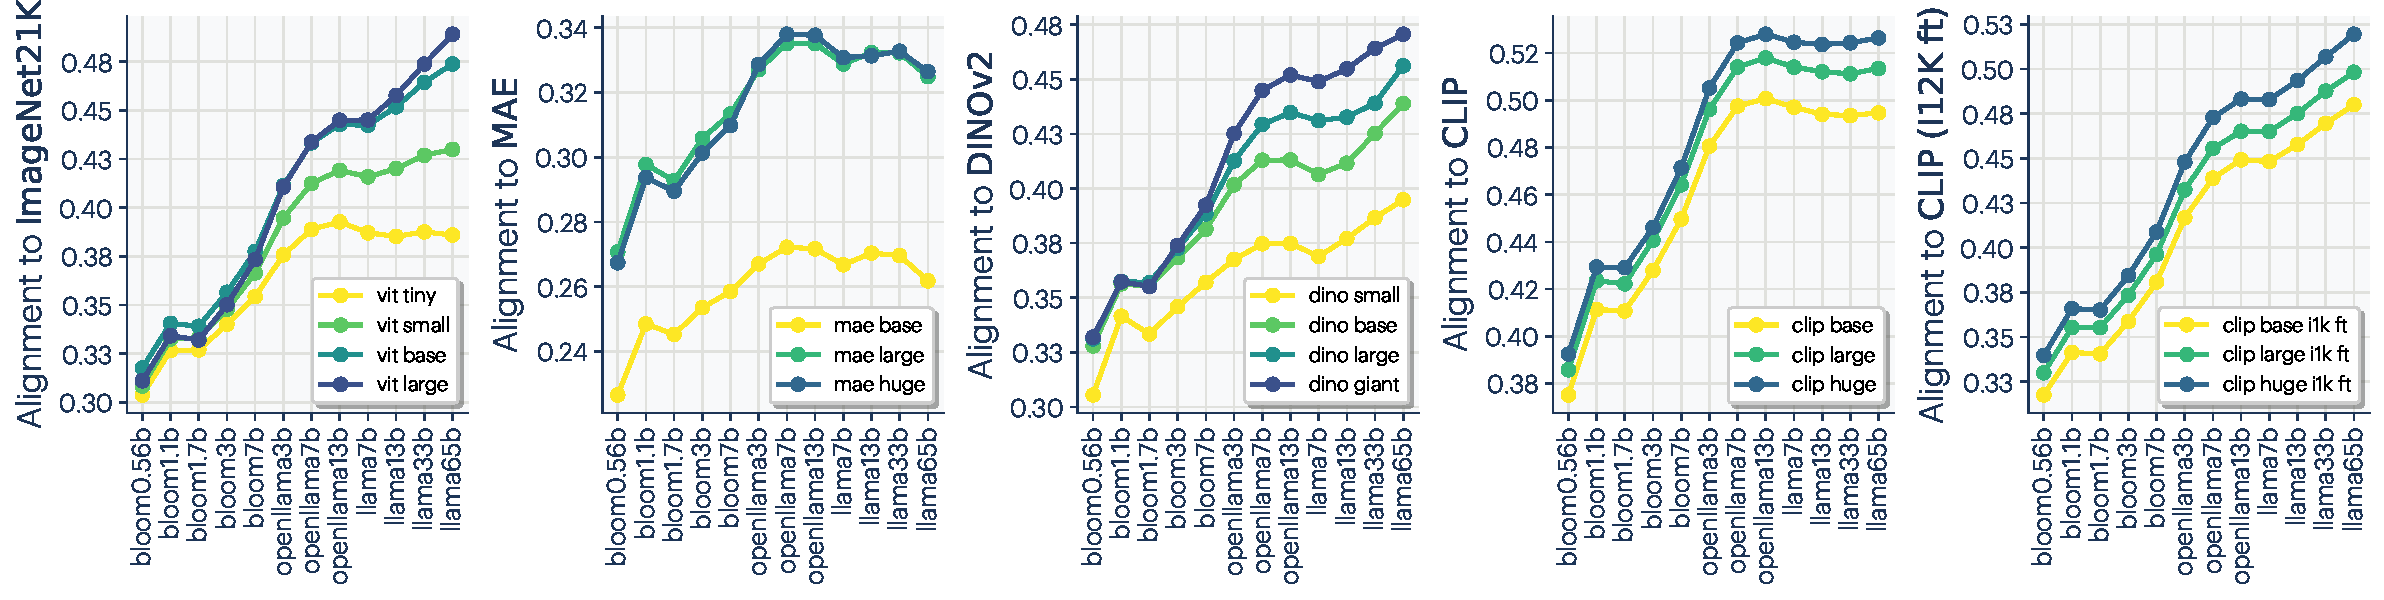
\includegraphics[width=1.0\linewidth]{figures/metrics_biased_cka.pdf}
    }\\
    \subfigure[Unbiased CKA]{
        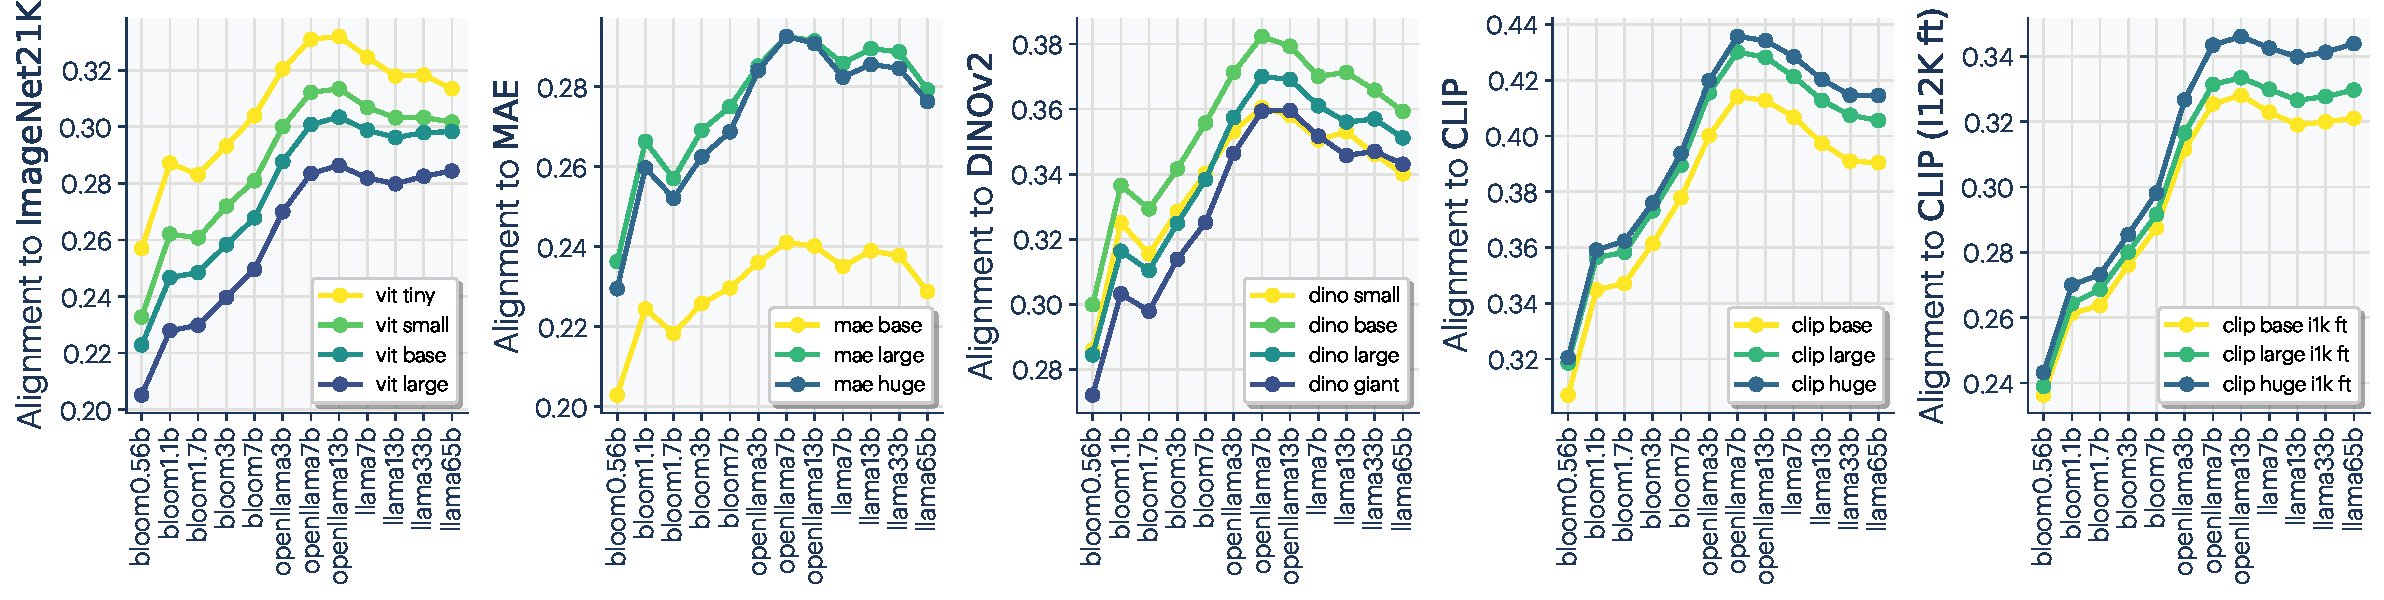
\includegraphics[width=1.0\linewidth]{figures/metrics_cka.pdf}
    }\\
    \subfigure[SVCCA]{
        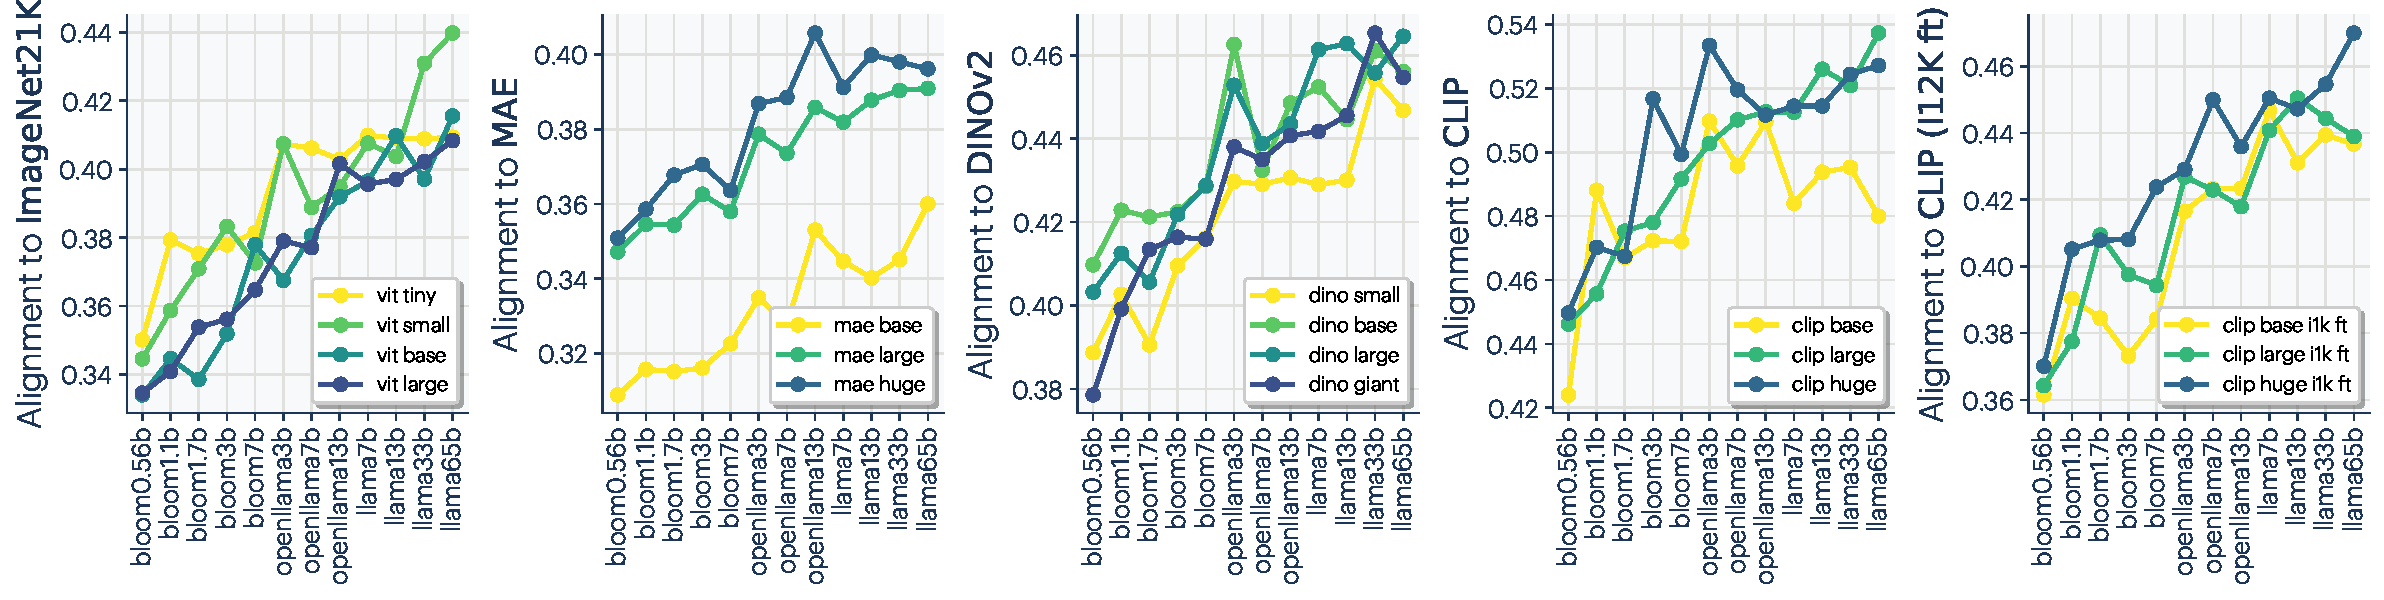
\includegraphics[width=1.0\linewidth]{figures/metrics_svcca.pdf}
    }\\
    \subfigure[Mutual $k$-NN ($k=10$)]{
        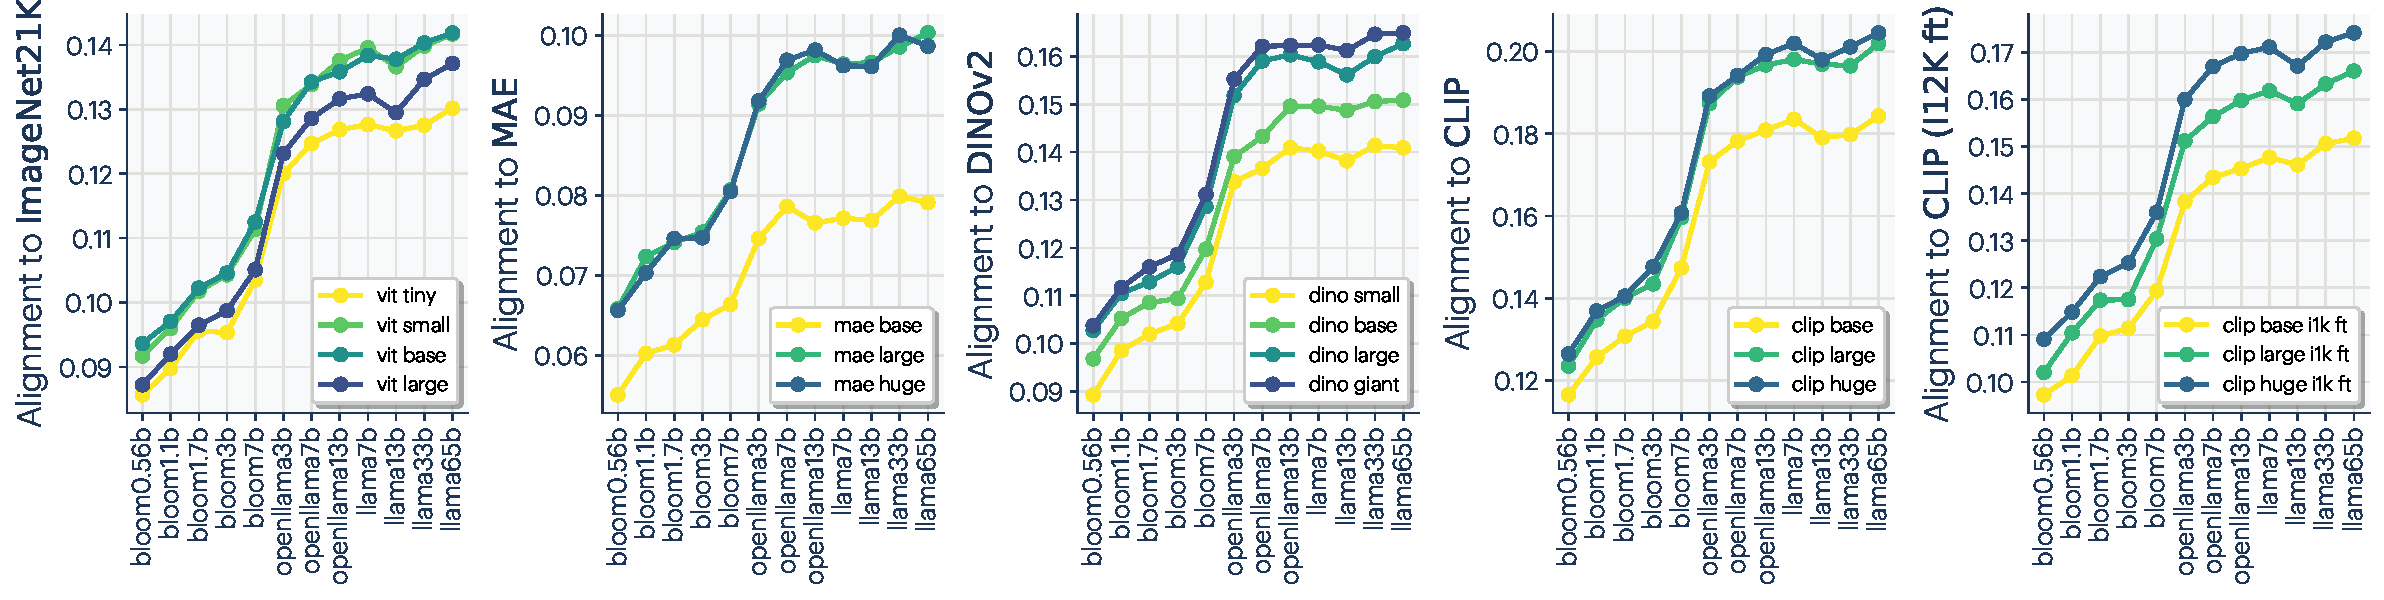
\includegraphics[width=1.0\linewidth]{figures/metrics_mutual_knn10.pdf}
    }
    \caption{\textbf{Cross-modal alignment for various metrics}}
    \label{fig:metrics1of2}
\end{figure*}

\begin{figure*}[hbtp]
    \centering
    \subfigure[CKNNA ($k=10$)]{
        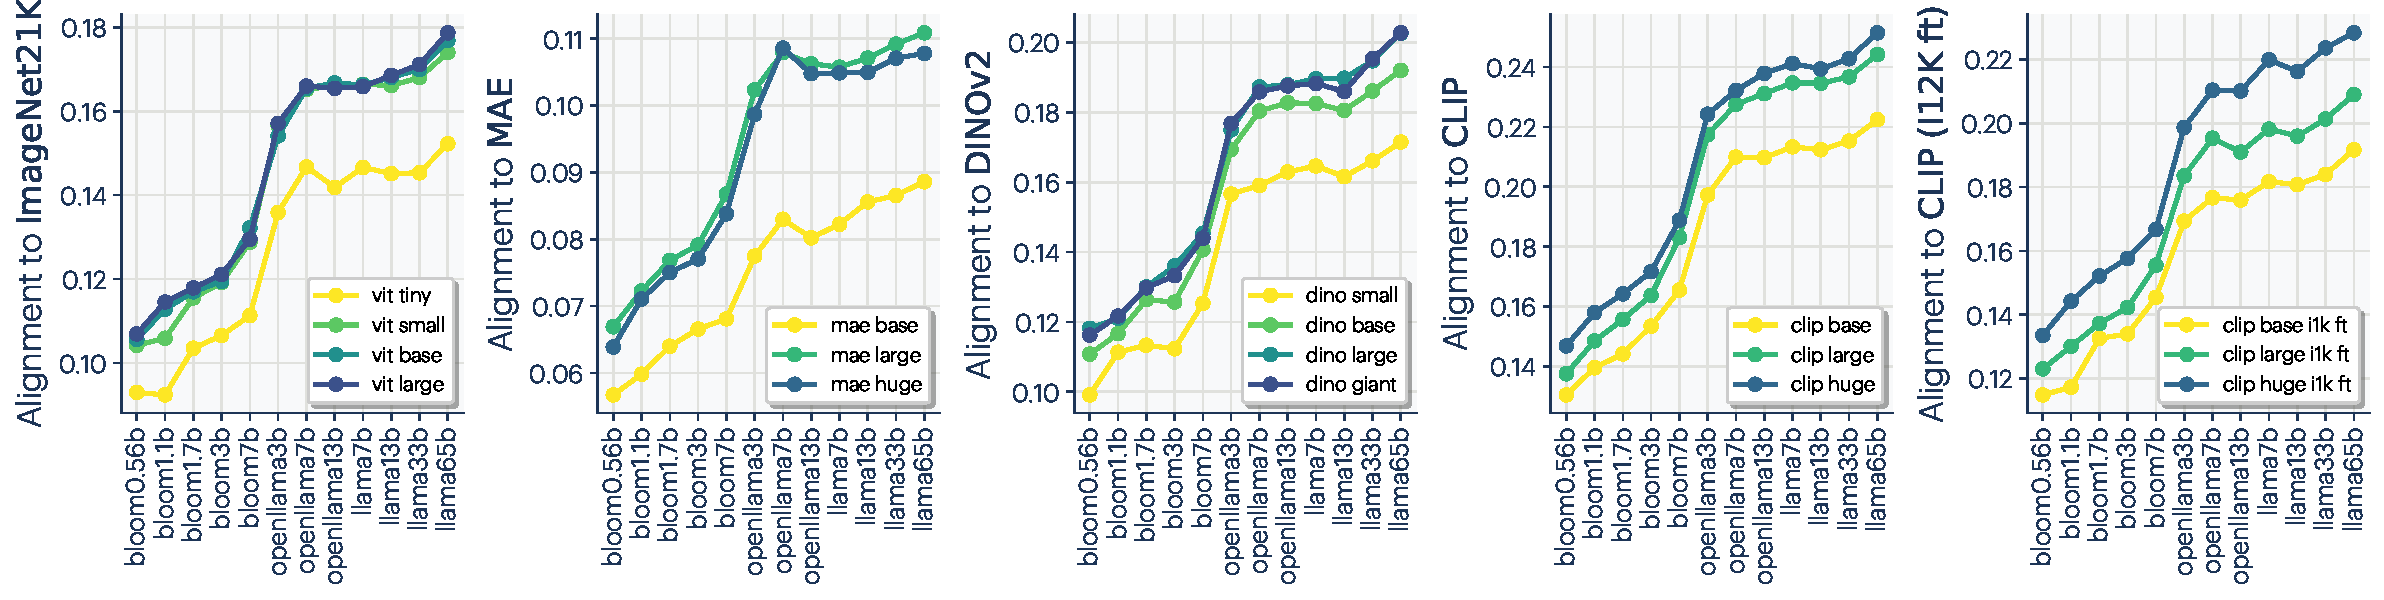
\includegraphics[width=1.0\linewidth]{figures/metrics_cknna10.pdf}
    }
    \subfigure[Cycle $k$-NN ($k=10$)]{
        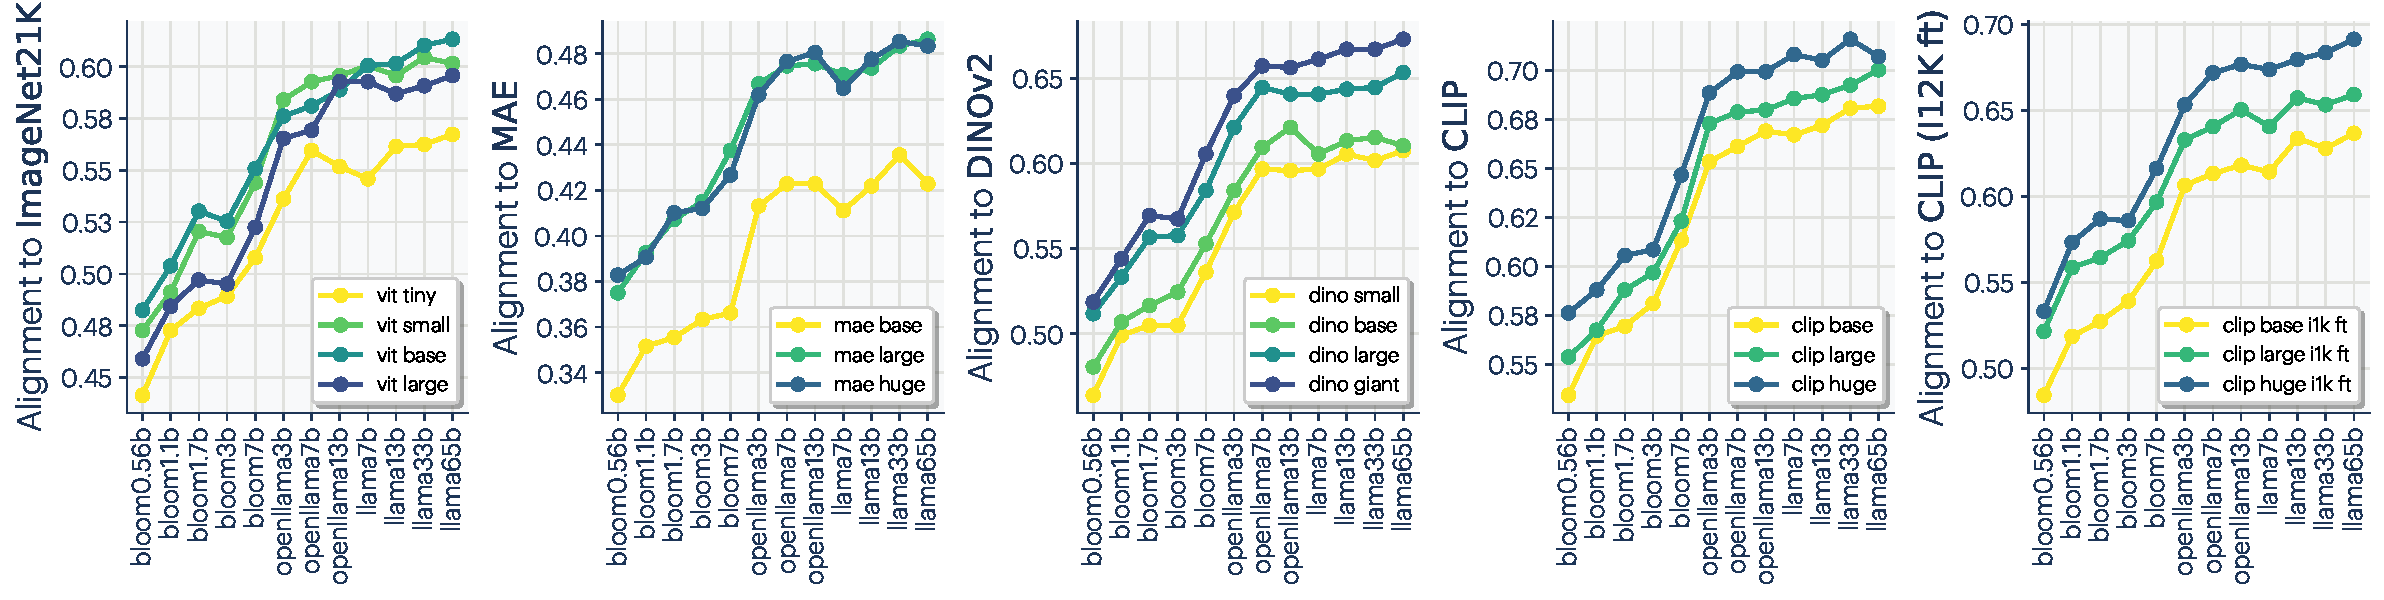
\includegraphics[width=1.0\linewidth]{figures/metrics_cycle_knn10.pdf}
    }\\
    \subfigure[Edit-distance $k$-NN ($k=10$)]{
        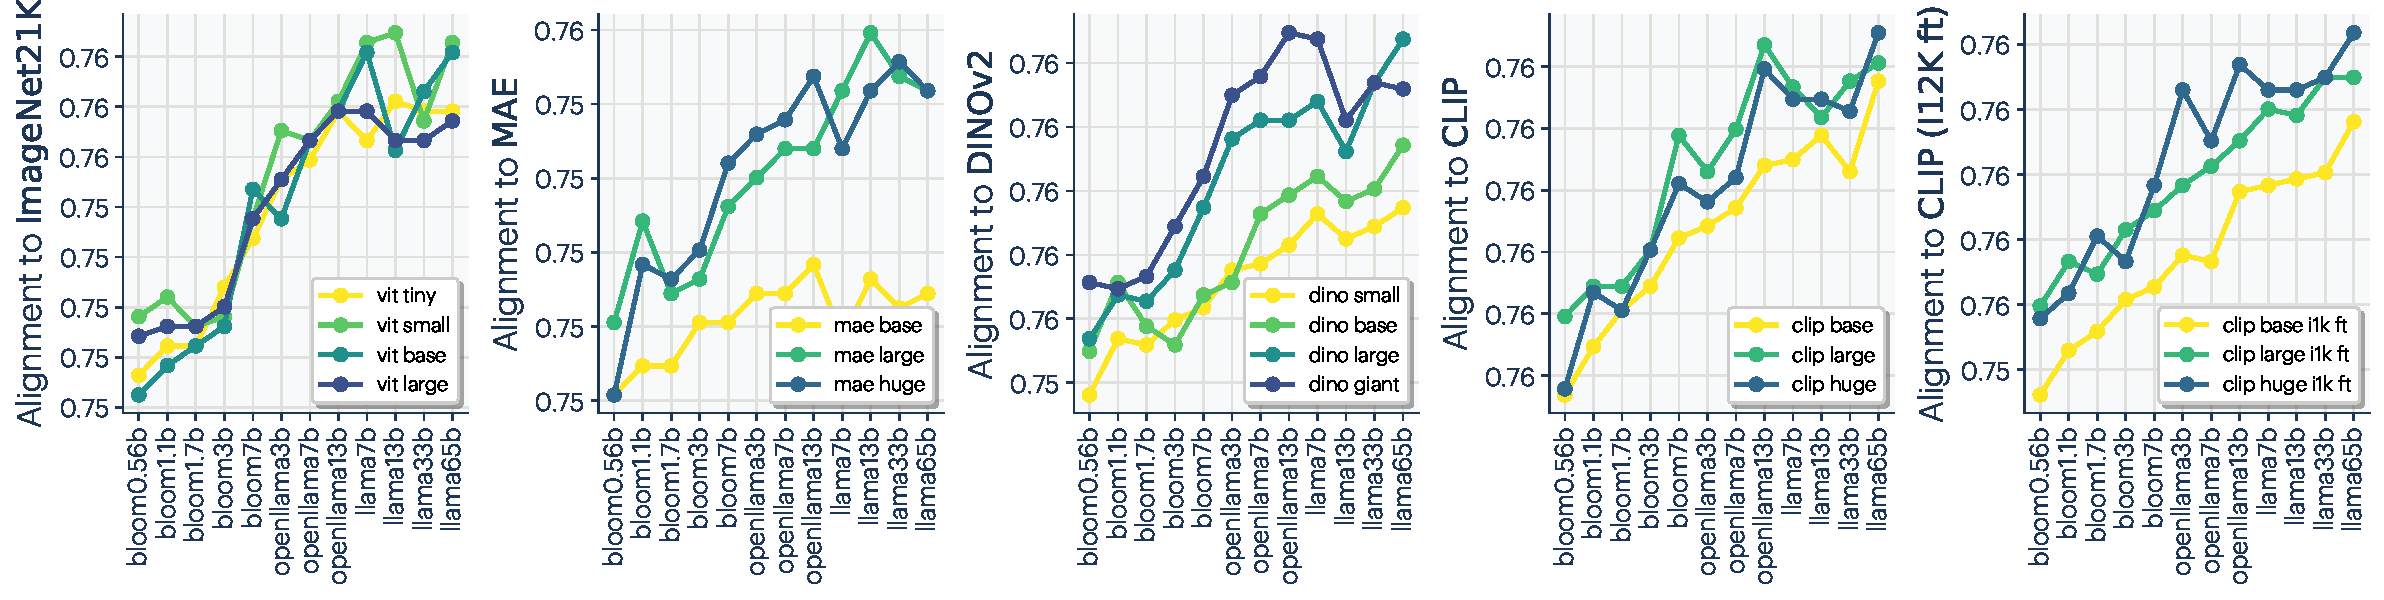
\includegraphics[width=1.0\linewidth]{figures/metrics_edit_distance_knn10.pdf}
    }\\
    \subfigure[Longest-Common-Subsequence $k$-NN ($k=10$)]{
        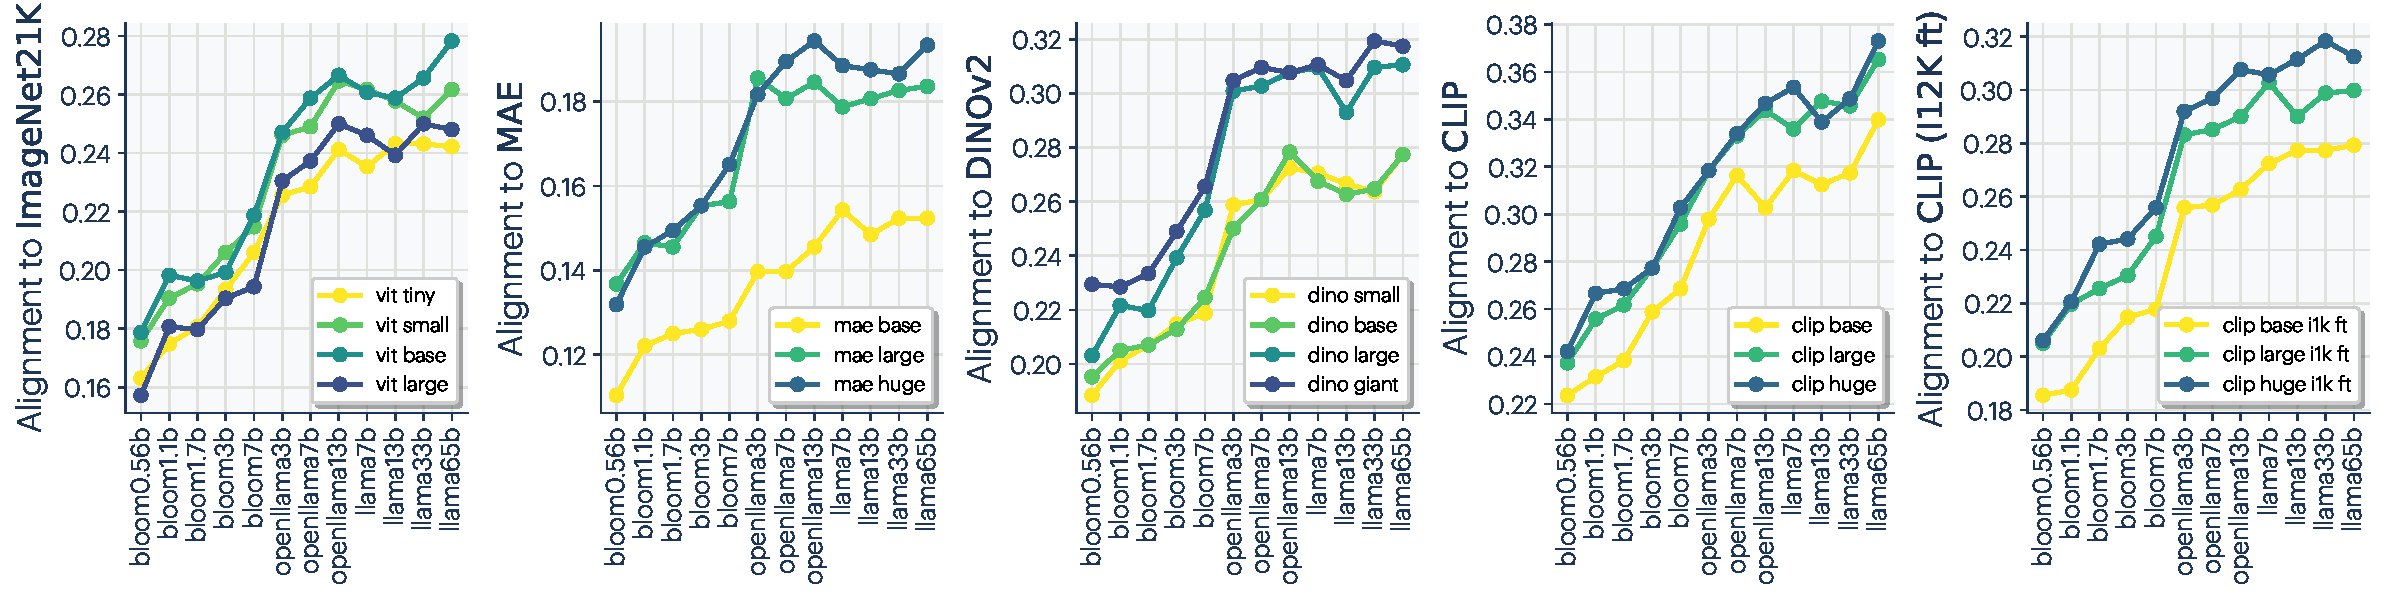
\includegraphics[width=1.0\linewidth]{figures/metrics_lcs_knn10.pdf}
    }
    \caption{\textbf{Cross-modal alignment measured with various metrics}}
    \label{fig:metrics2of2}
\end{figure*}

\newpage
\section{Experiments on Evaluating Alignment and Convergence}
\label{sec:alignment_methods}

To demonstrate representational convergence, we take off-the-shelf models at multiple scales and multiple modalities and measure their representational alignment. 

\subsection{Vision-Vision Alignment and Representation Quality}
\label{sec:vision-vision-details}

We consider 78 vision models in total: \begin{itemize}
    \item $17$ ViT models ranging from ViT-tiny to ViT-giant, trained on tasks including ImageNet-21k~\cite{dosovitskiy2020image} classification, Masked Autoencoders~\cite{he2021masked}, DINO~\cite{caron2021emerging}, and CLIP~\cite{radford2021learning}, including some finetuned on ImageNet-12k. 
    
    \item $1$ randomly initialized ResNet-50.
    \item $11$ ResNet-50 models trained with contrastive learning on ImageNet-1k, Places-365 \citep{zhou2017places,lopez2020semantic}, and $9$ synthetic image datasets used in \citet{baradad2022procedural}.  
    \item $49$ ResNet-18 models trained with Alignment and Uniformity contrastive loss \citep{tongzhouw2020hypersphere} on ImageNet-100, Places-365, and $47$ realistic and synthetic image datasets from \citet{baradad2021learning}.
\end{itemize}
% We used 16 of the 17 vision models used cross-modal alignment, skipping DINO ViT-gigantic due to its expensive compute requirement. In addition, we used 1 randomly initialized ResNet-50, 11 ResNet-50 models trained with contrastive learning on various realistic and synthetic datasets from \citet{baradad2022procedural}, and 49 ResNet-18 models trained with Alignment and Uniformity contrastive loss \citep{tongzhouw2020hypersphere} on various realistic and synthetic image datasets from \citet{baradad2021learning}. 

To test representation quality, we evaluate linear probing performance on all 19 VTAB classification tasks \citep{zhai2019vtab}, which is a standard multi-task transfer learning benchmark containing structured, specialized, and natural datasets covering diverse domains. To reduce compute requirements, we subsample training and validation datasets to have at most 10{,}000 samples. We consider a representation solves a task if its performance is $\geq 80\%$ of the best performance on that task across all 78 models. 

% To compute the alignment metric, we use $k=95$ nearest neighbors over $19\times512$ image representations, with $512$ images coming from each VTAB task's validation dataset, where $k$ is chosen such that on average $10$ images are considered as nearest neighbors for every $1024$ candidates.

To compute the alignment metric, we use $k=10$ nearest neighbors over $1000$ image representations computed on Places-365's validation dataset \citep{zhou2017places}. This dataset is disjoint from VTAB datasets, although both contain natural images.

\subsection{Cross-Modal Alignment}
\label{sec:vision-language-details}

% Our method begins with an analysis of cross-modal similarity. 
We compare the representation of an image in a vision model to the representation of a caption describing that image in a language model. The language model families we consider are BLOOM~\cite{bigscience2022bloom}, OpenLLaMA~\cite{openlm2023openllama}, and LLaMA~\cite{touvron2023llama}.
For~\fig{fig:downstream}, we included more recent model families such as OLMo~\cite{groeneveld2024olmo}, LLaMA3~\cite{meta2024llama3}, Gemma~\cite{team2024gemma}, and Mistral/Mixtral~\cite{jiang2023mistral,jiang2024mixtral}. These models were downloaded from Huggingface~\cite{wolf2019huggingface}.

For vision models, we consider ViT models~\cite{dosovitskiy2020image} of various sizes trained on various data and objectives. We mainly consider the popular vision models: classification on ImageNet-21K~\cite{russakovsky2015imagenet}, MAE~\cite{he2021masked}, DINOv2~\cite{oquab2023dinov2}, CLIP~\cite{radford2021learning}, and CLIP finetuned on ImageNet-12K. These models were downloaded from PyTorch Image Models~(TIMM; \citet{timm}). This is a subset of the models used in vision-vision comparison.

% In the vision domain, we consider $17$ models, including $17$ ViT models used in vision-vision alignment experiment detailed above.
% architectures that range from ViT-tiny to ViT-gigantic and tasks including ImageNet-1k~\cite{dosovitskiy2020image}, Masked Autoencoders~\cite{he2021masked}, DINO~\cite{caron2021emerging} and CLIP~\cite{radford2021learning} and CLIP finetuned on ImageNet-1k. 

% We compare language and vision models on 4 datasets with varying degrees of semantic coverage: ImageNet-1k~\cite{}, COCO Captions, and WIT (Wikipedia-based Image Text).  

To compute the alignment metric, we use $k=10$ nearest neighbors over 1024 samples from WIT (Wikipedia-based Image Text; \citet{srinivasan2021wit}). For the vision model, we use class token of each layer, and for the language model, we average pool each layer to a single token. Since it is not trivial to determine where the alignment might occur, we draw inspiration from BrainScore\cite{schrimpf2018brain} and compute pairwise alignment scores, then take the maximum. One of these pairwise comparisons also includes concatenated features. We apply $l_2$ normalization to the features before measuring the distance. As transformer architectures have ``emergent outliers''~\cite{dettmers2022gpt3}, we truncate the elements in the features that are above the $95$-th percentile.

Simply taking the last token did not show any strong alignment signal. We also experimented with prompting the language model and taking the last token representation. The prompt we used was 
\begin{align*}
    \texttt{An image with the caption `{<caption>}'. This is an image of a <fill>}
\end{align*}
Using prompting showed similar trends to average pooling but had slightly lower alignment scores.

% Move closer  to section 3 (remove the part in Section 2) and reference to appendix for more details, should not be longer than a paragraph. Results secotion 3.3, we had to run multimodal experiments and describe results here.


% \paragraph{Nearest Neighbor Overlap Metric}
% We measure the alignment between the representations of two models by looking at the percentage overlap between the nearest neighbor sets of the embeddings of two models for a given datapoint. The higher the overlap, the higher the alignment score. Furthermore, we add the constraint that the overlap must be \emph{ordinal}, the overlap requires the order of closest examples to be the same.

% CKA too strong of an alignment.
% Non-isotropic scaling can easily break CKA.
% Two models that have the same ordinal structure but slightly different distances between clusters can also break it.
% How do we compute distance that is more lax
% But the ordinal structuring seems to be aligning. 
% The nearest neighbors of a point


% \begin{figure*}[t!]
%     \centering
%     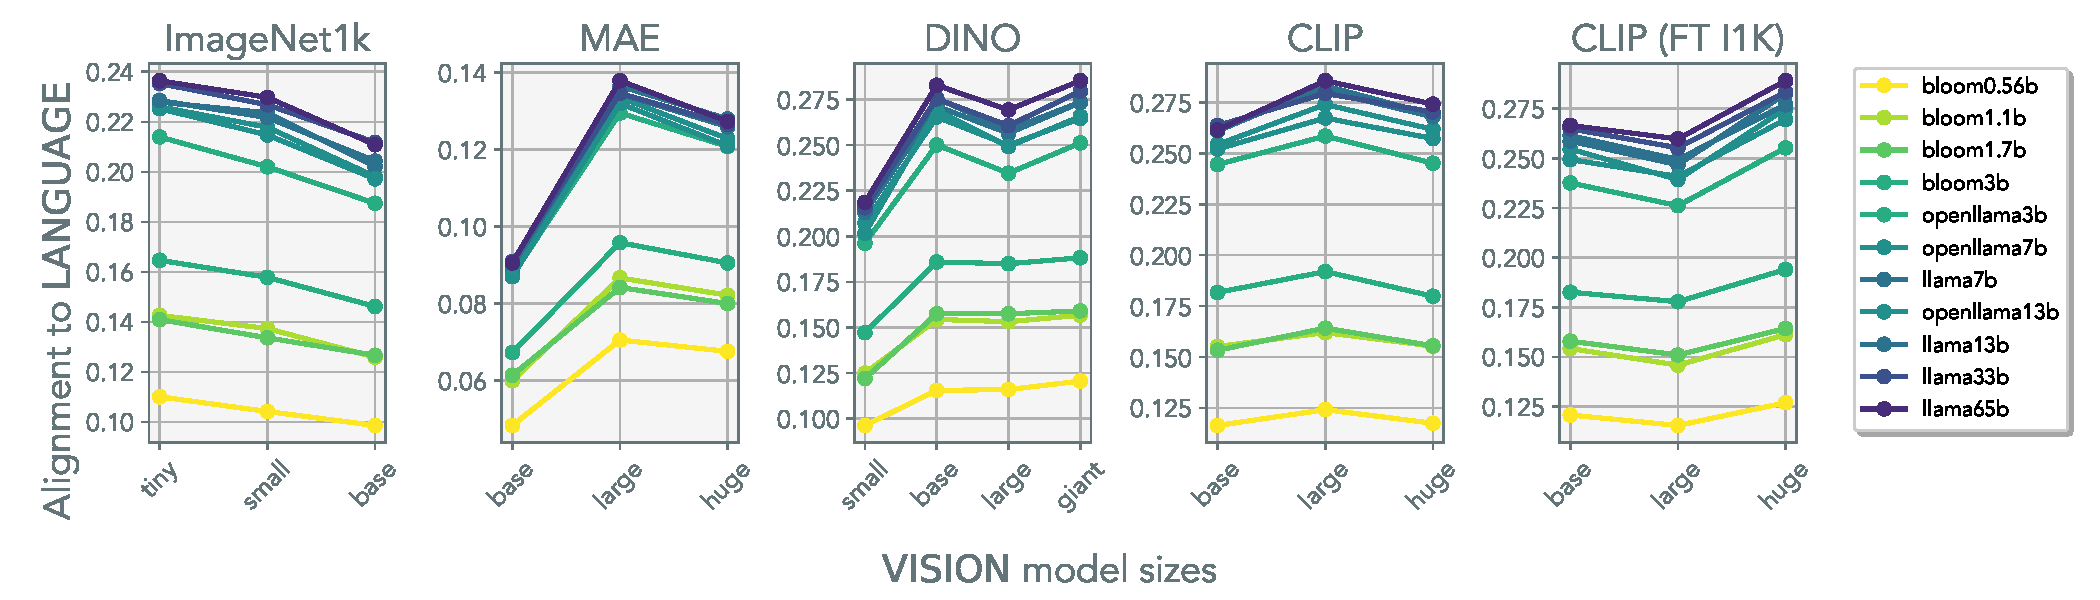
\includegraphics[width=1.\linewidth]{figures/lvm_alignment_per_task_imagenet1k.pdf}
%     \vspace{-0.2in}
%     \caption{\small \textbf{Vision-language alignment on ImageNet1k}}
%     \label{fig:llm2lvm_align}
% \end{figure*}


% \begin{figure*}[t!]
%     \centering
%     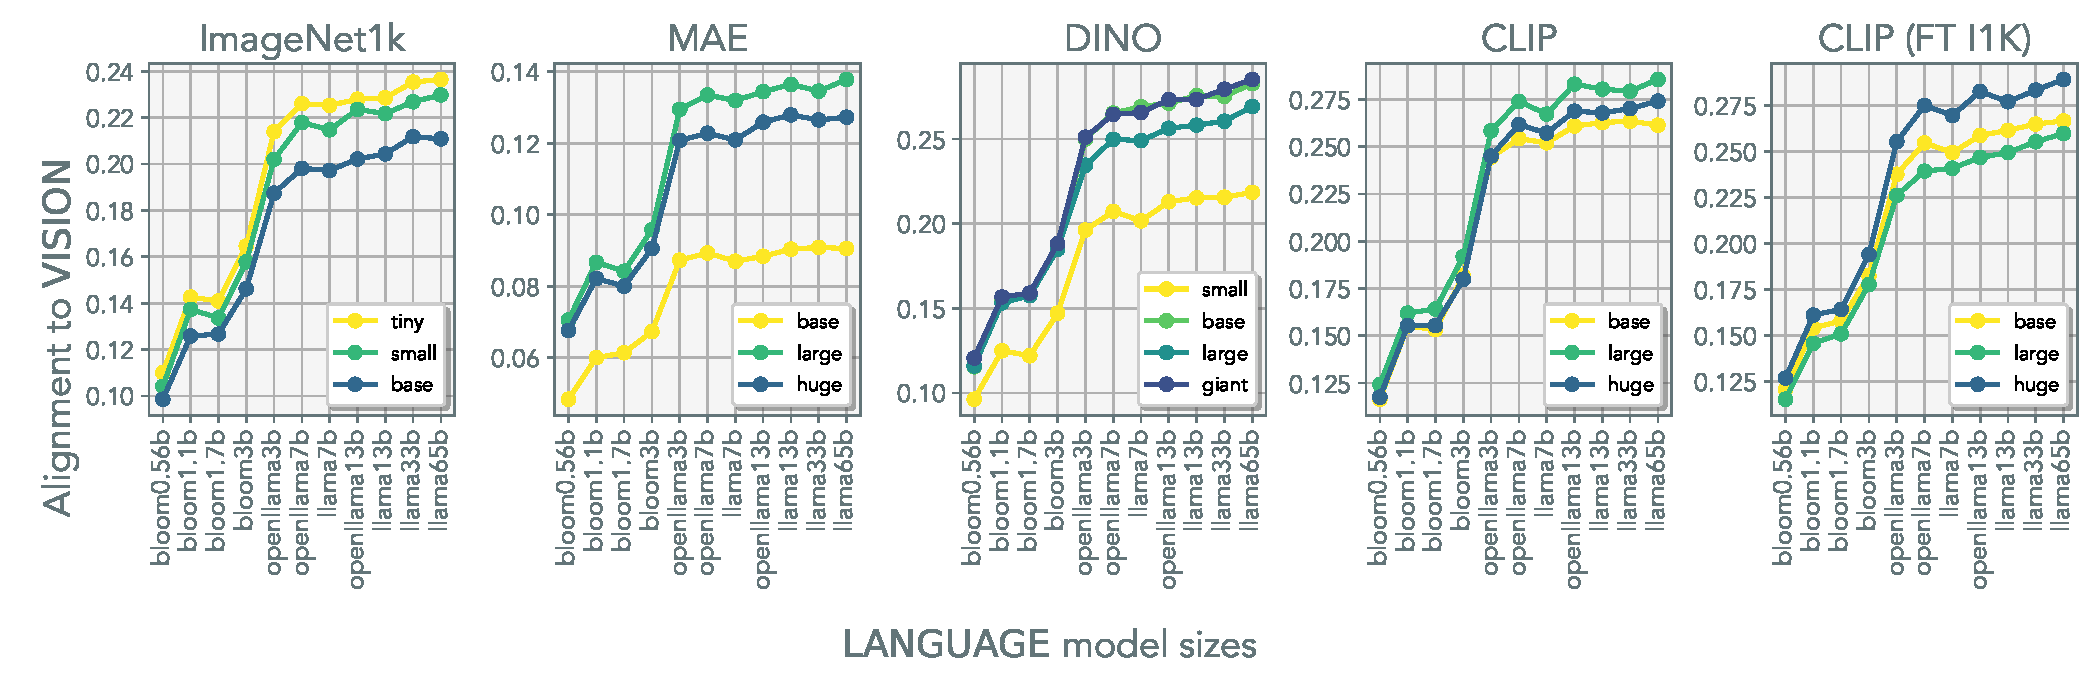
\includegraphics[width=1.\linewidth]{figures/llm_alignment_per_task_imagenet1k.pdf}
%     \vspace{-0.2in}
%     \caption{\small \textbf{Language-vision alignment on ImageNet1k}}
%     \label{fig:llm2lvm_align}
% \end{figure*}

% \begin{figure*}[t!]
%     \centering
%     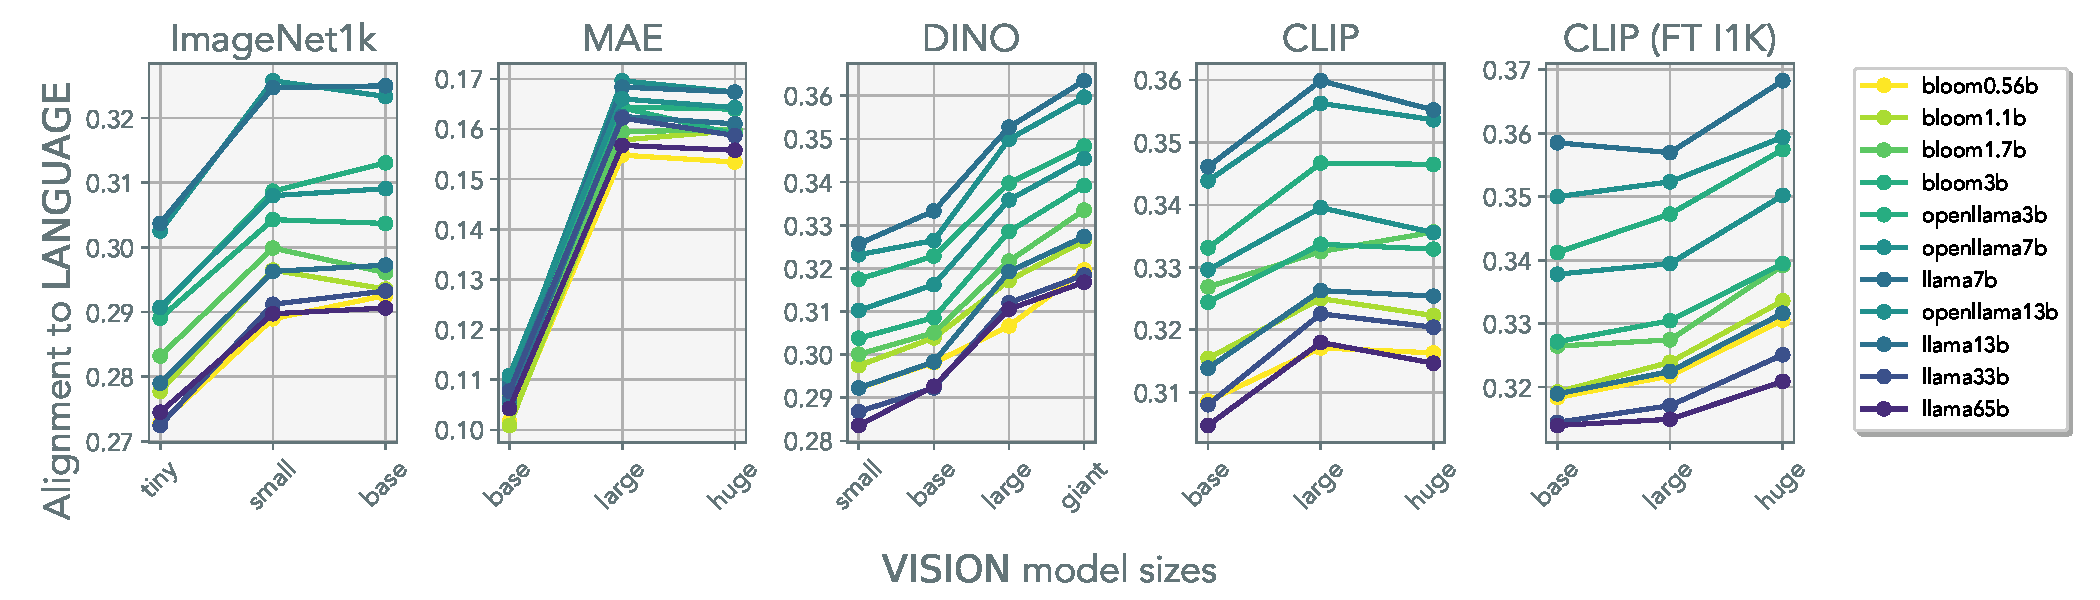
\includegraphics[width=1.\linewidth]{figures/lvm_alignment_per_task_coco.pdf}
%     \vspace{-0.2in}
%     \caption{\small \textbf{Vision-language alignment on COCO}}
%     \label{fig:llm2lvm_align}
% \end{figure*}

% \begin{figure*}[t!]
%     \centering
%     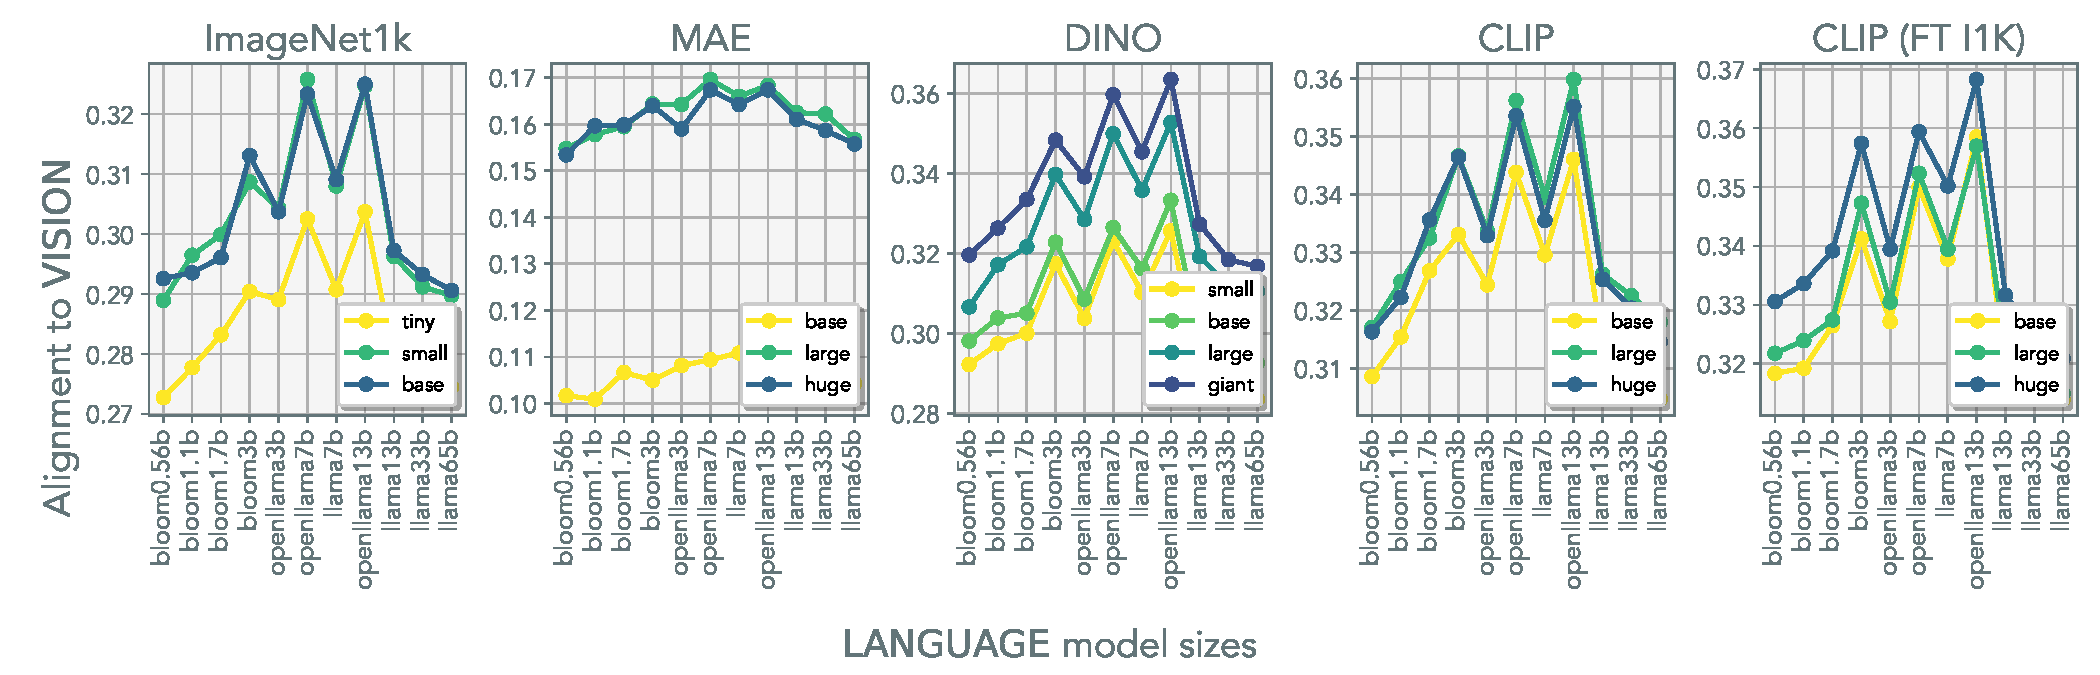
\includegraphics[width=1.\linewidth]{figures/llm_alignment_per_task_coco.pdf}
%     \vspace{-0.2in}
%     \caption{\small \textbf{Language-vision alignment on COCO}}
%     \label{fig:llm2lvm_align}
% \end{figure*}


\section{Color Cooccurrence Experiment}
\label{sec:color_cooccurrences}

Here we describe the details of how we created the four color representations visualized in \Cref{fig:color_pAB}, from left to right.

\paragraph{Perceptual representation from CIELAB color space} We embed pixels taken from the CIFAR-10 image dataset \citep{krizhevsky2009learning,torralba200880} based on the CIELAB color space, which is designed as a \emph{perceptually uniform} space that changes numerical values correspond to similar perceived changes in color.

\paragraph{Three representations from cooccurrence in VISION and LANGUAGE}
For these three representations, we first obtain a dissimilarity matrix over colors (in different ways detailed below), then use multidimensional scaling~\citep{shepard1980multidimensional} to find a 3-dimensional embedding in which Euclidean distance between the embeddings for $A$ and $B$, ${z}_A$ and ${z}_B$, best matches this dissimilarity matrix. We use $1{,}000$ fits and take the best match. Afterward, we visually align it with the CIELAB space by finding the best rotation, translation, scaling, and flipping, by running the Kabsch-Umeyama algorithm \citep{kabsch1976solution,kabsch1978discussion,umeyama1991least} twice, once on $\mathbf{z}$ and once on $-\mathbf{z}$, to account for flipping. The dissimilarity matrix we used in each case is described as following:\begin{itemize}
    \item \textbf{VISION: Pixel cooccurrence.} 
    We collect color cooccurrence statistics from the CIFAR-10 dataset, and estimate a joint distribution $p(A,B)$ over $300{,}000$ randomly sampled pixel colors $A$ and $B$ that occur within a radius of at most 4 pixels of one another. Colors are quantized on a grid in RGB space and represented as discrete variables, and $p(A,B)$ is modeled as a table of normalized counts, from which we compute the empirical pointwise mutual information matrix $\Kpmi(A, B)$. Quantization ensures that there is no bias from how color distances are represented in RGB space. Dissimilarity matrix is defined as $-\Kpmi(A, B) + c$, where $c = \max_{A, B} \Kpmi(A, B)$ is an offset to ensure non-negativity (similar to the constant in \Cref{sec:simple-contra-kpmi} and \Cref{prop:kpmi-psd-scale} that ensures neural networks can express $\Kpmi$).
    \item \textbf{LANGUAGE.} We used an approach similar to \citet{abdou2021can}.  \begin{itemize}
        \item We take $20$ pairs of (color, word) appeared in the dataset collected by \citet{lindsey2014color}, where $51$ participants were asked to free name each of the $330$ colors from the Munsell Color Chart. We filtered words that appeared less than $100$ times, and computed each word's associate color by taking the centroid in CIELAB space. Our filtering process followed \citet{abdou2021can} exactly, but resulted in $20$ colors, a slightly different set than the $18$ colors they claimed. 
        \item For each of the $20$ color words $\texttt{<col>}$, we construct three sentences: \begin{align*}
            & \texttt{The color <col>.} \\
            & \texttt{This color is <col>.} \\
            & \texttt{The color of this thing is <col>.}
        \end{align*}
        and obtain the average sentence embedding from the language encoder, as the embedding for $\texttt{<col>}$ (details below). We find this approach more effective than \citet{abdou2021can}, which uses object names that potentially have color biases, even though the objects may appear in multiple colors.
        \item Unlike \citet{abdou2021can}, we did not perform linear regression from language embedding to CIELAB space, which distorts distances and easily overfits with only $20$ samples. Instead, we used multidimensional scaling to best preserve distances, as described above.
        \item \textbf{Masked language contrastive learning (SimCSE) embedding: }
        We used sentence embedding from the unsupervised SimCSE RoBERTa-L \citep{gao2021simcse} to encode the above sentences into $1024$-dimensional embeddings, and used the pairwise Euclidean distances among $\texttt{<col>}$ embeddings as the dissimilarity matrix.
        \item \textbf{Masked language predictive learning (RoBERTa) embedding: }
        We concatenated hidden states of the last four layers of RoBERTa-L \citep{liu2019roberta}, following \citep{devlin2018bert}. We averaged across token dimensions, and obtained a $4096$-dimensional embedding for each of the above sentences, and used the pairwise Euclidean distances among $\texttt{<col>}$ embeddings as the dissimilarity matrix.
    \end{itemize}
\end{itemize}

\section{Caption Density Experiments}
\label{sec:caption_density}
We use LLaMA3-8B-Instruct~\cite{meta2024llama3} to generate summary captions at various densities for images in the Densely Captioned Images dataset~\cite{urbanek2023picture} from the train split. Following ~\citet{urbanek2023picture}, we prompt the language model with the following instructions to generate captions at differing granularity:

\texttt{system: You are given a full-text description of an image. You should summarize it into about <num\char`_words> words, being sure to include as much salient visual information as possible given the <num\char`_words> word constraint, especially information from the start of the original description. The new description should apply for the original image. Respond with only the summary, in one line.}

\texttt{user: <original\char`_caption>}

We measure the alignment with this generated caption to test our hypothesis that denser captations would result in higher alignment scores. In~\Cref{fig:caption_density}, we find that the alignment score also improves as caption length increases.

\section{Analysis of Contrastive Learners}\label{sec:analysis_contrastive}

\subsection{Contrastive objectives learn pointwise mutual information}\label{sec:analysis_contrastive-pmi}

There are two widely used forms of contrastive objectives. We now discuss each form in detail and show how they both are minimized by the pointwise mutual information (PMI) as stated in \Cref{eqn:contr-pmi}. To simplify notation, we consider learning the bivariate model $g(x_a, x_b) \in \mathbb{R}$. In \Cref{sec:what_rep},  such $g$ is optimized within the family of $\{g = \langle f_X, f_X \rangle \colon f_X \in \mathcal{F}_X\}$. 

Recall that our positive pairs are sampled from $(x, x_+) \sim \Pco$, and that the negative pairs are sampled independently from its marginals which we denote as $(x, x_-) \iidsim P$ where  $P(x) = \sum_{x_+} \Pco(x, x_+)$.
\begin{enumerate}
    \item \textbf{The binary NCE loss \citep{gutmann2010noise}} is defined with a certain prior over sampling positive vs.~negative pairs. Let $p_\mathsf{pos}$ be the probability of sampling a positive pair. Then the loss is given by \begin{equation}
        \mathcal{L}_\mathsf{binary\mbox{-}NCE}(g) 
        \trieq p_\mathsf{pos} \cdot \mathbb{E}_{(x, x_+) \sim \Pco}\left[ -\log \sigma(g(x, x_+)) \right]
        + (1 - p_\mathsf{pos}) \cdot \mathbb{E}_{(x, x_-) \iidsim P}\left[ -\log \sigma(-g(x, x_-)) \right].
    \end{equation}

    The Bayes optimal solution is given by \begin{align}
        g(x_a, x_b) 
        & = \log \frac{P(\texttt{pos} \given x_a, x_b)}{1 - P(\texttt{pos} \given x_a, x_b)} \\
        & = \log \frac{P(\texttt{pos}, x_a, x_b)}{P(\texttt{neg}, x_a, x_b)} \\
        & = \log \frac{p_\mathsf{pos} \cdot \Pco(x_a, x_b)}{(1 - p_\mathsf{pos}) P(x_a) P(x_b)} \\
        & = \log \frac{\Pco(x_a, x_b)}{P(x_a)P(x_b)} + \log \frac{p_\mathsf{pos}}{1 - p_\mathsf{pos}} \\
        & = \Kpmi(x_a, x_b) + c_X.
    \end{align}
    \item \textbf{The InfoNCE loss \citep{oord2018representation}} is defined with randomly sampling one positive pair along with $K$ negative ones. With some hyperparameter $\tau > 0$, the loss is given by \begin{equation}
        \mathcal{L}_\mathsf{InfoNCE}(g) 
        \trieq \mathbb{E}_{\substack{(x, x_+) \sim \Pco \\ (x_-^{(1)}, x_-^{(2)}, \dots, x_-^{(K)}) \iidsim P}}\left[ -\log \frac{e^{g(x, x_+) / \tau}}{e^{g(x, x_+) / \tau} + \sum_{i=1}^K e^{g(x, x_-^{(i)}) / \tau}} \right].
    \end{equation}

    The Bayes optimal solution is given by \begin{align}
        \frac{e^{g(x, x_+) / \tau}}{e^{g(x, x_+) / \tau} + \sum_{i=1}^K e^{g(x, x_-^{(i)}) / \tau}}
        & = \frac{\Pco(x_+ \given x) \prod_j P(x_-^{(j)}) }{\Pco(x_+ \given x) \prod_j P(x_-^{(j)})  + \sum_i \Pco(x_-^{(i)} \given x) P(x_+) \prod_{j \neq i} P(x_-^{(j)})} \\
        & = \frac{\Pco(x_+ \given x) / P(x_+) }{\Pco(x_+ \given x) / P(x_+) + \sum_i \Pco(x_-^{(i)} \given x) / P(x_-^{(i)})}.
    \end{align}

    For $\tau = 1$, this optima corresponds to $g$ choices where \begin{align}
        g(x_a, x_b) 
        & = \log \frac{\Pco(x_b \given x_a)}{P(x_b)} + c_X(x_a) \\
        & = \Kpmi(x_a, x_b) + c_X(x_a).
    \end{align}

    For the general $\tau \neq 1$ case, we have $g$ (and corresponding $f_X$) recovers $\Kpmi$ up to an offset and a scale. Our main argument in \Cref{sec:what_rep} that $f_X$ recovers $\Kpmi$ still holds.
\end{enumerate}

\subsection{Contrastive learners can represent $\Kpmi$ exactly under smoothness conditions}
\label{sec:analysis_contrastive-exact-repr}


% \paragraph{Contrastive learners} Contrastive learners align positive samples and push apart negative samples. Often positive samples are defined as two cooccurring observations. In this setting, contrastive learning is intimately related to modeling the coccurrence probability $P(x^1,x^2)$~\cite{XX,YY,ZZ}. We will show this for the particular case of the InfoNCE objective~\cite{XX}:
% \begin{align}
%     InfoNCE
% \end{align}
% The minimizer of this objective is:
% \begin{align}
%     e^{-f_X(x^1)^T f_X(x^2)} &\propto \frac{P(x^1 | x^2)}{P(x^1)}\\
%     &= \frac{e^{-K_{\texttt{cooccur}}(x^1,x^2)}}{P(x^1)P(x^2)}
% \end{align}

% \paragraph{Predictive learners}
% \begin{align}
%     e^{-f_X(x)^T f_Y(y)} &\propto P(y | x)\\
%     &= \frac{e^{-K_{\texttt{cooccur}}(x,y)}}{P(x)}
% \end{align}

% This suggests that contrastive and predictive learners should converge to somewhat different representations. However, both are related to the cooccurrence kernel. We conjecture that the denominators do not have a large effect in practice. That is, a strong form of the platonic representation hypothesis is that all these objectives -- modeling cooccurrences directly, contrastive learning, predictive learning -- converge on roughly the same kernel, up to constant scale and shift. This would strictly be the case if all the marginals are uniform distributions, since in that case the denominators become constants. Perhaps variation in the numerator swamps variation in the denominator, making the uniformity assumption be approximately valid in practice.



% \begin{proposition}
%     Suppose that $\Pcoij$ is bounded below by $\delta$ and that the events $z_i$ are in a non-degenerate discrete space $\mathcal{Z}$ with $\size{\mathcal{Z}} \geq 2$. Then $\Kpmi + C$ is positive semi-definite for some constant $C = -\log \delta$ if $\pcoor$ is sufficiently smooth (or that the sampling frequency is high enough) so that \begin{equation}
%         % \PcoiCi \geq 1 - \frac{4}{9} N (N-1) \delta^2, \mathrlap{\qquad \forall i.}
%         \PcoiCi \geq  \frac{1}{1 + N(N-1)\delta^2}\mathrlap{\qquad \forall i.}
%     \end{equation}
% \end{proposition}

% \begin{proof}
%     Note that our event space is discrete, so \begin{equation}
%         \Kij = \log \Pcoij - \log \Pcoi - \log \Pcoj \geq \log \Pcoij.
%     \end{equation}
%     Then we know that $\Kpmi - \log \delta$ is a $N \times N$ symmetric matrix with non-negative entries. Then it suffices to show that it is diagonally dominant in the following sense: $\forall i$, \begin{align}
%         && 
%         \log \Kii - \log \delta 
%         & \geq \sum_{j \neq i} \Kij - (N - 1) \log \delta \notag\\
%         %
%         & \iff &
%         \log \PcoiCi \underbrace{{}- \log \Pcoi}_{\geq 0} + (N - 2) \log \delta 
%         & \geq  \underbrace{\sum_{j\neq i} \log \PcojCi}_{\mathclap{\leq (N - 1) \log \frac{1 - \PcoiCi}{N-1}}}  + \underbrace{\vphantom{\sum_{j}}(-\log \Pcoj)}_{\mathclap{\leq - \log N \delta\vphantom{\frac{\PcojCi}{N}}}} \notag\\
%         %
%         & \impliedby &
%         \log \PcoiCi + (N-1) \log N(N-1) + (2N-3)\log \delta & \geq  (N - 1) \log (1 - \PcoiCi) \notag\\
%         %
%         & \iff &
%         \frac{1}{N-1} \underbrace{\log \PcoiCi}_{\leq 0} + \log N(N-1) + (2 - \frac{1}{N-1}) \underbrace{\log \delta}_{< 0} & \geq \log (1 - \PcoiCi) \notag\\
%         %
%         & \impliedby &
%         \log \PcoiCi + \log N(N-1) + 2 \log \delta & \geq \log (1 - \PcoiCi) \notag\\
%         %
%         & \iff &
%         \frac{1 - \PcoiCi}{\PcoiCi} \leq  N(N-1)\delta^2 \notag \\
%         % . \label{eqn:final-cot}
%         %
%         & \iff &
%         \PcoiCi \geq  \frac{1}{1 + N(N-1)\delta^2}.
%     \end{align}

%     From this, one can already derive a reasonable condition where large enough $\PcoiCi$ makes \Cref{eqn:final-cot} hold. Since the goal of this analysis is to show the overall idea, rather than to find the best bound, we make a few more relaxations to obtain a simple linear form.

%     Note that $\delta \leq N^{-2}$. So for $N \geq 2$, RHS of \Cref{eqn:final-cot} has \begin{equation}
%         N(N-1)\delta^2 \leq N (N - 1) / N^4 \leq \frac{1}{8}.
%     \end{equation}

%     Consider LHS of \Cref{eqn:final-cot}. Observe that $f(p) \trieq \frac{1-p}{p}$ is convex and monotonically decreasing over $p \in (0, 1]$, reaching $0$ at $p=1$. Hence, it is sufficient to consider the region where $f(\PcoiCi) \leq \frac{1}{8}$, that is $\PcoiCi \in [\frac{8}{9}, 1]$. Over this region, we have $f(\PcoiCi) \leq \frac{9}{8} (1 - \PcoiCi)$.

%     Therefore, with $N \geq 2$, \Cref{eqn:final-cot} holds when \emph{both} of the following hold: \begin{align}
%         \PcoiCi & \geq \frac{8}{9} \label{eqn:final-cond1}\\
%         \frac{9}{8} (1 - \PcoiCi ) & \leq N(N-1)\delta^2. \label{eqn:final-cond2}
%     \end{align}

%     Note that both hold when \begin{equation}
%         \PcoiCi \geq 1 - \frac{4}{9} N (N - 1) \delta^2. \label{eqn:final-single-cond}
%     \end{equation}

%     \begin{itemize}
%         \item \Cref{eqn:final-cond2} is satisfied since \begin{equation}
%             1 - \frac{4}{9} N (N - 1) \delta^2 \geq 1 - \frac{8}{9} N (N - 1) \delta^2.
%         \end{equation}

%         \item \Cref{eqn:final-cond1} is satisfied since \begin{equation}
%             1 - \frac{4}{9} N (N - 1) \delta^2 \geq 1 - \frac{4}{9} N^{-2} \geq 1 - \frac{1}{9} (\frac{2}{N})^2 \geq 1 - \frac{1}{9} = \frac{8}{9}.
%         \end{equation}
%     \end{itemize}

%     Hence, \Cref{eqn:final-single-cond} is a sufficient condition.
% \end{proof}

We want to express $\Kpmi + C$ using some representation function $f_X \colon \mathcal{X} \rightarrow \mathbb{R}^n$ so that \begin{equation}
    \langle f_X(x_a), f_X(x_b) \rangle = \Kpmi(x_a, x_b) + C, \qquad\text{for some $C$.}
\end{equation}For such an $f_X$ to exist, an equivalent criterion is that $\Kpmi + C$ is positive semi-definite (PSD), as can be seen from eigendecomposition.

\begin{proposition}\label{prop:kpmi-psd-scale}
    Suppose that the off-diagonal elements of $\Kpmi$ are bounded within $[\log \rho_\mathsf{min}, \log \rho_\mathsf{min} + \delta] \in (-\infty, 0]$. We have $\Kpmi + C$ is positive semi-definite (PSD) for some $C$ if the joint distribution is sufficiently smooth: \begin{equation}
        \frac{\PcoiCi}{\Pcoi} \geq e^{N \delta} \rho_\mathsf{min}\mathrlap{,\qquad \forall i.}
    \end{equation}
\end{proposition}

\begin{proof}

    Note that $\Kpmi +C$ still only has non-positive off-diagonal elements if \begin{equation}
        - C \geq \log \rho_\mathsf{min} + \delta. \label{eq:C-cond}
    \end{equation}
    For such $C$, it is diagonally dominant (and thus PSD) if, \begin{equation}
        \mathllap{\forall i,\qquad} \Kii +C \geq \sum_{j\neq i} \abs{\Kij + C} = - (N - 1) C - \sum_{j\neq i} \Kij,
    \end{equation}
    or equivalently, \begin{equation}
        \mathllap{\forall i,\qquad} NC + \sum_j \Kij \geq 0.\label{eq:diag-dom-sufficient}
    \end{equation}
    
    The following choice of $C$ readily satisfies the above \Cref{eq:diag-dom-sufficient}: \begin{equation}
        C \trieq -\min_i \frac{1}{N} \sum_j \Kij. 
    \end{equation}

    Therefore, it remains to show that \Cref{eq:C-cond} is true.  Note that \begin{equation}
        - C \trieq \min_i \frac{1}{N} \sum_j \Kij \geq \frac{N-1}{N} \log \rho_\mathsf{min} + \frac{1}{N} (\min_i \Kii). 
    \end{equation}

    Therefore, it suffices to have \begin{equation}
        \log \rho_\mathsf{min} + \delta \leq \frac{N-1}{N}  \log \rho_\mathsf{min} + \frac{1}{N} (\min_i \Kii). 
    \end{equation}
    Rearranging terms gives the desired condition \begin{equation}
    % L_\mathsf{diag} \geq \underbrace{N \cdot \log U_\mathsf{off} - (N - 1) \log L_\mathsf{off}}_{\geq 0}.
    \frac{\PcoiCi}{\Pcoi} \geq e^{N \delta} \rho_\mathsf{min}\mathrlap{,\qquad \forall i.}
    \end{equation}
\end{proof}
\begin{remark}
\Cref{prop:kpmi-psd-scale} is one example that a sufficiently smooth world or a sufficiently high sampling rate allows the PMI kernel $\Kpmi$ to be \emph{exactly} represented as inner products of a learned feature space (up to a scale). The condition here can be satisfied, for example, if the off-diagonal terms decay linearly with respect to $N$ and stay sufficiently close to each other. While the condition is somewhat strict, it 
captures the essence that smoothness and continuity allow easier learning. Nonetheless, we note that exact representation is not necessary for convergence, and thus this requirement can likely be relaxed.  Please see \Cref{sec:limitations} for discussions on practical settings.
\end{remark}

% \begin{proof}
%     Denote with $\rho$ the maximum marginals: \begin{equation}
%         \rho \trieq \max_i \Pcoi  \geq 1/N.
%     \end{equation}

%     Then we have $\forall i$, \begin{align}
%         \frac{\PcoiCi}{\Pcoi} 
%         & = \frac{1}{\Pcoi} \bigg(1 - \sum_{j \neq i} \frac{\PcojCi}{\Pcoj} \Pcoj\bigg) \\
%         & \geq \frac{1}{\rho} \bigg(1 - \sum_{j \neq i} U_\mathsf{off} \rho\bigg) \\
%         & = \frac{1}{\rho} - (N-1) U_\mathsf{off}.
%     \end{align}

%     Hence we can pick $L_\mathsf{diag} = \frac{1}{\rho} - (N-1) U_\mathsf{off}$. Then \Cref{eq:diag-cond} reduces to \begin{align}
%         &&
%         \frac{1}{\rho} - (N-1) U_\mathsf{off} 
%         & \geq U^N_\mathsf{off} / L^{N-1}_\mathsf{off} \\
%         \iff &&
%         \frac{1}{U_\mathsf{off}} & \geq (x^{N-1}+N-1)\rho
%     \end{align}
% \end{proof}


% \section{Additional implications}

% \paragraph{Training models to align could improve performance}

% \paragraph{Information-dense sensors might be useful}

% \phil{It should help to create richer caption datasets because with max info in language you should converge to platonic visual rep...}